%\footnote{See supplementary material for an enlarged version of this figure}
\vspace{-0.5cm}
\section{Methods}\label{sec:methods}
A more detailed analysis of the local linear model reveals that it is closely related to the CC matching functional. Although the tendency of CC to fit a (global) linear model to the joint PDF is well known and has been previously pointed out by other authors (see for example Hermosillo {\it et al.} \cite{Hermosillo2004}), in this section we describe the underlying model from which the (local) CC functional is obtained, then we extend the model to account for multi-modal images, and finally we show an efficient way to incorporate the resulting matching functional into the SyN transformation model.

\subsection{Relationship between LLR and CC}
To establish the relationship between LLR and CC, consider the non-degenerate case first (the case that $\mathbf{y}_{\mathbf{v}}$ and $\mathbf{x}_{\mathbf{v}}$ are not ``constant'' vectors or in other words, they are not scalar multiples of $\mathbbm{1}$), we will discuss the degenerate cases later. \textcolor{red}{For any positive integer $k$ and any vector $\mathbf{z}\in \mathbbm{R}^{k}$, denote the centered vector $\mathbf{z}' = \mathbf{z} - \frac{\mathbbm{1}^{T}\mathbf{z}}{k}\mathbbm{1}_{k}$ with corresponding elements $z_{i}'=z_{i} - \frac{\mathbbm{1}^{T}\mathbf{z}}{k}, i=1,2,...,k$, and the normalized vector $\widehat{\mathbf{z}} = \frac{\mathbf{z}'}{||\mathbf{z}'||}$, where all entries of $\mathbbm{1}_{k}\in \mathbbm{R}^{k}$ are equal to $1$.} Note that we may assume, without loss of generality, that both vectors $\mathbf{x}_{\mathbf{v}}, \mathbf{y}_{\mathbf{v}}$ are \emph{centered} (i.e., their means are zero: $\frac{\mathbf{x}_{\mathbf{v}}^{T}\mathbbm{1}}{n} = \frac{\mathbf{y}_{\mathbf{v}}^{T}\mathbbm{1}}{n} = 0$) since the LLR evaluated at non-centered vectors equals the LLR evaluated at their corresponding centered vectors. Therefore, the projection matrix $\mathbf{Q}_{\mathbf{v}}$ in \eqref{eq:def_P_v} can be directly computed as
%, which may be proven as follows. Decompose $\mathbf{x}_{\mathbf{v}}, \mathbf{y}_{\mathbf{v}}$ into their centered part and their mean: $\mathbf{x}_{\mathbf{v}} = \mathbf{x}_{\mathbf{v}}' + \mu_{x}\mathbbm{1}$, and $\mathbf{y}_{\mathbf{v}} = \mathbf{y}_{\mathbf{v}}' + \mu_{y}\mathbbm{1}$. Then
%\begin{displaymath}
%    \begin{array}{lcl}
%        ||[\mathbf{x}_{\mathbf{v}} \; \mathbbm{1}]\boldsymbol{\beta} - \mathbf{y}_{\mathbf{v}}||^{2} &=& ||[\mathbf{x}_{\mathbf{v}}' \; \mathbbm{1}]\boldsymbol{\beta} - \mathbf{y}_{\mathbf{v}}' + \beta_{1}\mu_{x}\mathbbm{1} - \mu_{y}\mathbbm{1}||^{2}\\
%        &=&||[\mathbf{x}_{\mathbf{v}}' \; %\mathbbm{1}]\boldsymbol{\tilde{\beta}} - \mathbf{y}_{\mathbf{v}}'||^{2}
%    \end{array}
%\end{displaymath}
%where $\boldsymbol{\tilde{\beta}} = (\beta_{1}, \beta_{0} + \beta_{1}\mu_{x} - \mu_{y})^{T}$. This $\boldsymbol{\tilde{\beta}}$ is the unique maximum likelihood estimator for $\boldsymbol{\beta}$ in the centered, non-degenerate case. 
\begin{align*}
    \mathbf{Q}_{\mathbf{v}} &= [\mathbf{x}_{\mathbf{v}} \; \mathbbm{1}]
    \left[\begin{array}{cc}
        \frac{1}{||\mathbf{x}_{\mathbf{v}}||^{2}} & 0\\
        0 & \frac{1}{n}
    \end{array}\right]
    \left[\begin{array}{c}
        \mathbf{x}_{\mathbf{v}}^{T}\\
        \mathbbm{1}^{T}
    \end{array}\right]
\end{align*}
where $||\mathbf{x}_{\mathbf{v}}||^{2}$ cannot be zero, by hypothesis. Therefore, entry $q_{i,j}$ of $\mathbf{Q}_{\mathbf{v}}$ at row $i$, column $j$ is given by:
\vspace{-0.3cm}
\begin{displaymath}
    q_{i,j} = \frac{nx_{\mathbf{v},i}x_{\mathbf{v}, j} + ||\mathbf{x}_{\mathbf{v}}||^{2}}{n||\mathbf{x}_{\mathbf{v}}||^{2}}.
\end{displaymath}
Each term of the LLR metric (corresponding to the local window centered at voxel $\mathbf{v}$) can be expanded as:
\begin{equation}\label{eq:llr_cc_relationship}
    \begin{split}
        ||(\mathbf{Q}_{\mathbf{v}} - \mathbbm{I}_{n})\mathbf{y}_{\mathbf{v}}||^{2} &= \sum_{i=1}^{n} \left(\sum_{j=1}^{n} q_{i,j} y_{\mathbf{v}, j} - y_{\mathbf{v},i}\right)^{2}\\
        &=\sum_{i=1}^{n}\left(\frac{\mathbf{x}_{\mathbf{v}}^{T}\mathbf{y}_{\mathbf{v}}}{||\mathbf{x}_{\mathbf{v}}||^{2}} x_{\mathbf{v}, i} - y_{\mathbf{v},i}\right)^{2} \\
        &= ||\mathbf{y}_{\mathbf{v}}||^{2}\left(1 - \frac{(\mathbf{x}_{\mathbf{v}}^{T}\mathbf{y}_{\mathbf{v}})^{2}}{||\mathbf{x}_{\mathbf{v}}||^{2}||\mathbf{y}_{\mathbf{v}}||^{2}}\right).
    \end{split}
\end{equation}
%&=||\mathbf{y}_{v}||^{2} - \frac{(\mathbf{x}_{v}^{T}\mathbf{y}_{v})^{2}}{||\mathbf{x}_{v}||^{2}}\\
Therefore, the LLR functional may be regarded as a modified CC functional with a bias towards making $||\mathbf{y}_{\mathbf{v}}'||$ \textcolor{red}{close to zero}. This bias may be removed from model \eqref{eq:wang_model} by normalizing $\mathbf{y}_{\mathbf{v}}'$:\\
\begin{equation}\label{eq:normalized_ll_model}
    \widehat{\mathbf{y}_{\mathbf{v}}} = \left[\mathbf{x}_{\mathbf{v}} \; \mathbbm{1}\right]\boldsymbol{\beta} + \eta(\mathbf{v}) \; \forall \mathbf{v}\in\Omega_{I},
\end{equation}
and we can see that likelihood maximization under model \eqref{eq:normalized_ll_model} is now equivalent to maximization of CC.\\

Regarding the degenerate cases, note that if $\mathbf{y}_{\mathbf{v}} = \alpha \mathbbm{1}, \alpha\in \mathbbm{R}$, then the LLR at $\mathbf{v}$ is zero regardless of the value of $\mathbf{x}_{\mathbf{v}}$, otherwise, if $\mathbf{x}_{\mathbf{v}} = \gamma \mathbbm{1}, \gamma\in \mathbbm{R}$, then the LLR at $\mathbf{v}$ is $||\mathbf{y}_{\mathbf{v}}'||^{2}$, which confirms that the a registration algorithm driven by LLR has a bias towards making $\mathbf{y}_{\mathbf{v}}'$ \textcolor{red}{close to zero}. On the other hand, the CC metric is undefined in these degenerate cases (CC is defined for centered local vectors \cite{Avants2008}\cite{Avants2011}) and they are handled in practice by discarding their contribution to the metric and its gradient (this can be verified, for example, from the ANTS \cite{Avants2011a} source code).

\subsection{Global non-linear transfer}
The matching functional we propose in this work is based on the empirical observation that the non-linear relationship between both image modalities at local windows (Fig. \ref{fig:llr_test}) may be made closer to linear by applying a global, non-linear, transfer function $F: G \rightarrow \mathbbm{R}$ (Fig. \ref{fig:ecc_test_good}). More precisely, our model may be written as
\begin{equation}\label{eq:ecc_model}
\widehat{\mathbf{y}_{\mathbf{v}}} = \left[\mathbf{f_{v}} \; \mathbbm{1}\right]\boldsymbol{\beta} + \eta(\mathbf{v}) \; \forall \mathbf{v}\in\Omega_{I},
\end{equation}
where we have denoted $\mathbf{f_{v}} = F[\mathbf{x}_{\mathbf{v}}]$ the vector that results from applying function $F$ to each element of vector $\mathbf{x}_{\mathbf{v}}$. By following the exact same steps as before, we can compute the optimal regression parameters $\widehat{\boldsymbol{\beta}}$ and obtain the negative log-likelihood of our data under model \eqref{eq:ecc_model}, which is proportional to:
\begin{equation}\label{eq:ecc_neg_likelihood}
    U(I, J;\phi) = \sum_{\mathbf{v} \in \Omega_{I}} \left( 1 - \frac{(\mathbf{f_{v}'}^{T} \mathbf{y'}_{\mathbf{v}})^{2}}{||\mathbf{f_{v}'}||^{2}||\mathbf{y_{v}'}||^{2}}\right).
\end{equation}
The minimum of \eqref{eq:ecc_neg_likelihood} can be obtain by maximizing our proposed matching functional, which we call \emph{Expected Cross Correlation} (the reason of this name will be clear soon):
\begin{equation}\label{eq:ecc_functional}
    ECC(I, J;\phi) = \sum_{\mathbf{v} \in \Omega_{I}} \frac{(\mathbf{f_{v}'}^{T} \mathbf{y'}_{\mathbf{v}})^{2}}{||\mathbf{f_{v}'}||^{2}||\mathbf{y_{v}'}||^{2}}.
\end{equation}
\textcolor{red}{To compute an optimal transfer function, we need to write \eqref{eq:ecc_functional} in terms of the global $\mathbf{f}$. This may be accomplished by defining:}
%Now we will proceed to compute an optimal non-linear transfer function $F$. We can see from model \eqref{eq:ecc_model}, that the optimal function $F$ is not unique: if $F^{*}$ is optimal, then any affine transform of $F^{*}$, say $\tilde{F} = \alpha_{0} F^{*} + \alpha_{1}$ is optimal too, because:
%\begin{displaymath}
%    \left[\tilde{F}\left[\mathbf{x}_{\mathbf{v}}\right] \; \mathbbm{1}\right]\boldsymbol{\beta} =
%    \left[\left(\alpha_{0}F^{*}\left[\mathbf{x}_{\mathbf{v}}\right]+\alpha_{1}\mathbbm{1}\right) \; \mathbbm{1}\right]\boldsymbol{\beta} =
%    \left[F^{*}\left[\mathbf{x}_{\mathbf{v}}\right] \; \mathbbm{1}\right]\boldsymbol{\tilde{\beta}},
%\end{displaymath}
%where $\boldsymbol{\tilde{\beta}} = (\alpha_{0}\beta_{0}, \alpha_{1}\beta_{0} + \beta_{1})^{T}$. Let's denote by $m$ the number of different intensity values in the fixed image $I$ (a typical choice is $m=256$). We will assign a value $f_{\ell}$ to each intensity $\ell$ of the fixed image, $0\leq \ell < m$, and define the transfer function $F$ as $F(x_{\mathbf{v},i}) = f_{\ell}$, where $\ell = x_{\mathbf{v},i}$. The transfer function $F$ may then be represented as a vector $\mathbf{f}$ of dimension $m$. Let $k_{\mathbf{v},\ell}$, and $a_{\mathbf{v},\ell}$ be number of elements of $\mathbf{x}_{\mathbf{v}}$ equal to $\ell$, and the sum of elements of $\mathbf{y}_{\mathbf{v}}$ whose corresponding elements in $\mathbf{x}_{\mathbf{v}}$ equal $\ell$, respectively. More precisely:
\begin{displaymath}
	\begin{array}{lcl}
		k_{\mathbf{v},\ell} &=& |\left\lbrace i : x_{\mathbf{v},i}=\ell\right\rbrace|\\
		a_{\mathbf{v}, \ell} &=& \sum\limits_{i:x_{\mathbf{v},i}=\ell} y_{\mathbf{v},i}
	\end{array}\;\;\textcolor{red}{1\leq i \leq n, \;\; 1\leq \ell \leq m,}
\end{displaymath}
%\textcolor{red}{then, the dot product in equation \eqref{eq:ecc_neg_likelihood} may be written in terms of $\mathbf{f}$ as follows:
%\begin{displaymath}
%    \mathbf{f'_{v}}^{T} \mathbf{y}'_{\mathbf{v}} = \left[\sum_{\ell=1}^{m} f_{\ell}a_{\mathbf{v}, \ell}'\right] - \left(\frac{\mathbbm{1}^{T}\mathbf{f_{v}}}{n}\right) \mathbbm{1}^{T}\mathbf{y'_{v}} = \mathbf{f}^{T}\mathbf{a}'_{\mathbf{v}},
%\end{displaymath}}
%and the squared norm $||F[\mathbf{x}_{\mathbf{v}}]||^{2}$ as:
%\begin{displaymath}
%    ||F\left[\mathbf{x}_{\mathbf{v}}\right]||^{2} = \left[\sum_{\ell=1}^{m} f_{\ell}^{2} k_{\mathbf{v}, \ell}\right] - %\frac{\left(\mathbf{f}^{T}\mathbf{k_{v}}\right)^{2}}{n} = \mathbf{f}^{T} \left(\mathbf{D}_{\mathbf{v}} - \frac{1}{n}\mathbf{K_{v}}\right) \mathbf{f}
%\end{displaymath}
%where $\mathbf{D}_{\mathbf{v}} = $ diag($\mathbf{k}_{\mathbf{v}}$) and $\mathbf{K_{v}} = \mathbf{k_{v}}\mathbf{k}^{T}_{\mathbf{v}}$. The ECC matching functional \eqref{eq:ecc_functional} can now be written \textcolor{red}{ in terms of the global $\mathbf{f}$} as:
\textcolor{red}{and after some algebraic manipulations, \eqref{eq:ecc_functional} can be written as:
\begin{equation}\label{eq:ecc_neg_likelihood_vector_form}
    ECC(I, J;\phi) = \sum_{\mathbf{v} \in \Omega_{I}}\frac{\mathbf{f}^{T}\mathbf{a_{v}'}\mathbf{a_{v}'}^{T}\mathbf{f}}{\mathbf{f}^{T} \left[ \mathbf{D_{v}} - \frac{1}{n}\mathbf{K_{v}}\right]\mathbf{f} ||\mathbf{y_{v}'}||^{2}},
\end{equation}
where $\mathbf{D}_{\mathbf{v}} = $ diag($\mathbf{k}_{\mathbf{v}}$) and $\mathbf{K_{v}} = \mathbf{k_{v}}\mathbf{k}^{T}_{\mathbf{v}}$.} The problem of maximizing the sum of quotients of quadratic forms \eqref{eq:ecc_neg_likelihood_vector_form} does not have, in general, a close form solution, and it is necessary to resort to iterative algorithms \cite{Kiers1995}. The evaluation of the functional alone may be very time consuming because in order to apply fast strategies like \textcolor{red}{integral images \cite{Crow1984}\cite{Viola2004}\cite{Tapia2011}} we need to store the partial results for each intensity value $0 \leq \ell < m$, which would require a large amount of memory. Therefore, we will compute an approximation based on the following assumption:
\textcolor{red}{\begin{itemize}
    \item The set of intensity pairs $S_{\mathbf{v}}=\left\lbrace \left(x_{\mathbf{v}, i}, y_{\mathbf{v}, i}\right): 1\leq i \leq m\right\rbrace$ contained in each pair of local vectors $\mathbf{x}_{\mathbf{v}}$, $\mathbf{y}_{\mathbf{v}}$ is approximately a random sample from the full set of intensity pairs $S=\left\lbrace \left(I(\mathbf{v}), J(\phi(\mathbf{v}))\right): \mathbf{v}\in \Omega_{I}\right\rbrace$.
\end{itemize}}
%            \begin{equation*}
%                ||\mathbf{y}_{v}|| \approx ||F[\mathbf{x}_{v}]|| \; \forall v\in\Omega_{I}.
%            \end{equation*}
On the one hand, \textcolor{red}{under this condition,} the number $k_{\mathbf{v},\ell}$ of vector elements $i$ where $x_{\mathbf{v},i} = \ell$, may be approximated by its expected value $np_{\ell}$, where the probability $p_{\ell}$ of a voxel having intensity $\ell$ may be estimated by its empirical probability:
\begin{equation}
    \frac{k_{\mathbf{v}, \ell}}{n} \approx \frac{\mathbbm{E}[k_{\mathbf{v},\ell}]}{n} \approx \frac{|\left\lbrace \mathbf{v}\in\Omega_{I} : I(\mathbf{v}) = \ell\right\rbrace|}{|\Omega_{I}|} =: p_{\ell},
\end{equation}
and from this approximation it follows that $\frac{1}{n}\mathbf{D}_{\mathbf{v}} = \frac{1}{n}diag(\mathbf{k}_{\mathbf{v}}) \approx diag(\mathbf{p}) =: \mathbf{P}$.\\

On the other hand, the average $\frac{a_{\mathbf{v},\ell}}{k_{\mathbf{v},\ell}}$ of all elements of vector $\mathbf{y}_{\mathbf{v}}$ whose corresponding entries in $\mathbf{x}_{\mathbf{v}}$ are equal to $\ell$ may be approximated by the average computed over the full image $J$, where intensities in $I$ are equal to $\ell$:
\begin{equation}\label{eq:average_of_isosets}
    \frac{a_{\mathbf{v},\ell}}{k_{\mathbf{v},\ell}} =  \frac{1}{k_{\mathbf{v},\ell}}\sum_{i:x_{\mathbf{v},i}=\ell} y_{\mathbf{v},i} \approx \frac{1}{|G_{\ell}|}\sum_{\mathbf{v}\in G_{\ell}} J(\phi(\mathbf{v}))
    =:\bar{f}_{\ell},
\end{equation}
where $G_{\ell} = \left\lbrace \mathbf{v}\in \Omega_{I}: I(\mathbf{v}) = \ell\right\rbrace$. From the above conditions it follows that $\mathbf{a}_{\mathbf{v}} \approx n \mathbf{P} \mathbf{\bar{f}}$.\\

\textcolor{red}{By making the above approximations, it can be shown that the optimal transfer function is of the form $\mathbf{f^{*}} = \alpha_{0} \mathbf{\bar{f}} + \alpha\mathbbm{1}$, which implies that $\mathbf{\bar{f}}$ is optimal too, because:
\begin{displaymath}
    \left[\mathbf{f^{*}_{v}} \; \mathbbm{1}\right]\boldsymbol{\beta} = 
    \left[\left(\alpha_{0} \mathbf{\bar{f}} + \alpha_{1}\mathbbm{1}\right) \; \mathbbm{1}\right]\boldsymbol{\beta} =
    \left[\mathbf{\bar{f}} \; \mathbbm{1}\right]\boldsymbol{\tilde{\beta}},
\end{displaymath}
}
where $\boldsymbol{\tilde{\beta}} = (\alpha_{0}\beta_{0}, \alpha_{1}\beta_{0} + \beta_{1})^{T}$. The transfer function $\mathbf{\bar{f}}$ (defined by \eqref{eq:average_of_isosets}) is exactly the same as the optimal transfer function used in the CR and the EM matching functionals. As shown by Roche {\it et al.} \cite{Roche1998, Roche2000} and more recently by Arce {\it et al.} \cite{Arce-santana2014}, the transfer function $\mathbf{\bar{f}}$ evaluated over image $I$ corresponds to the conditional expectation of image $J$ given image $I$, more precisely:
\begin{equation*}
    F[I] = \mathbbm{E}[J | I]
\end{equation*}
where the expectation is evaluated point-wise (voxel by voxel) with respect to the conditional distribution of intensities of $J$ given intensities of $I$. Therefore:
\begin{equation}\label{eq:ecc_meaning}
    ECC(I, J; \phi) \textcolor{red}{\approx} CC(\mathbbm{E}[J|I], J ; \phi).
\end{equation}
from which we adopted the name ``Expected Cross Correlation''. Notice that, if the local windows $W_{\mathbf{v}}, \mathbf{v}\in\Omega_{I}$ are sufficiently large, then the condition we used to obtain \eqref{eq:ecc_meaning} from \eqref{eq:ecc_neg_likelihood_vector_form} are satisfied (to convince ourselves, it suffices to consider the extreme case of one single ``local'' window of size equal to the full volume). The question is how small the local windows can be so that this condition is reasonably satisfied. Please note that, in practice, we do not need this condition to be satisfied everywhere, but we only need that the optimal $\mathbf{f}$ obtained under the given assumptions is reasonably close to the optimal $\mathbf{f}$ obtained without making the assumption. From our experiments, as we will show below, we have found that rectangular local windows of radius $4$ voxels ($n=9\times 9\times 9 = 729$, the recommended default for the CC functional according to Avants {\it et al.} \cite{Avants2011}) work surprisingly well in practice.\\

To assess how reasonable our simplifying assumption is, we compared the optimal transfer function, computed by directly maximizing \eqref{eq:ecc_neg_likelihood_vector_form} w.r.t. $\mathbf{f}$ using BFGS \cite{GVK502988711}, and compared the result against the iso-set means $\mathbf{\bar{f}}$ (see Fig. \ref{fig:comparison_optimal_transfers}). We can see that regardless of the relatively small window sizes, the optimal transfers are very similar, which allows us to approximate the optimal transfer function (computationally very costly) with the iso-set means (fast and easy to compute). In Fig. \ref{fig:LLR_transfer_rmse} we show the norm of the difference between $\mathbf{\bar{f}}$ and the optimal transfer function as a function of the window size. \\

\begin{figure}[t]
\centering
    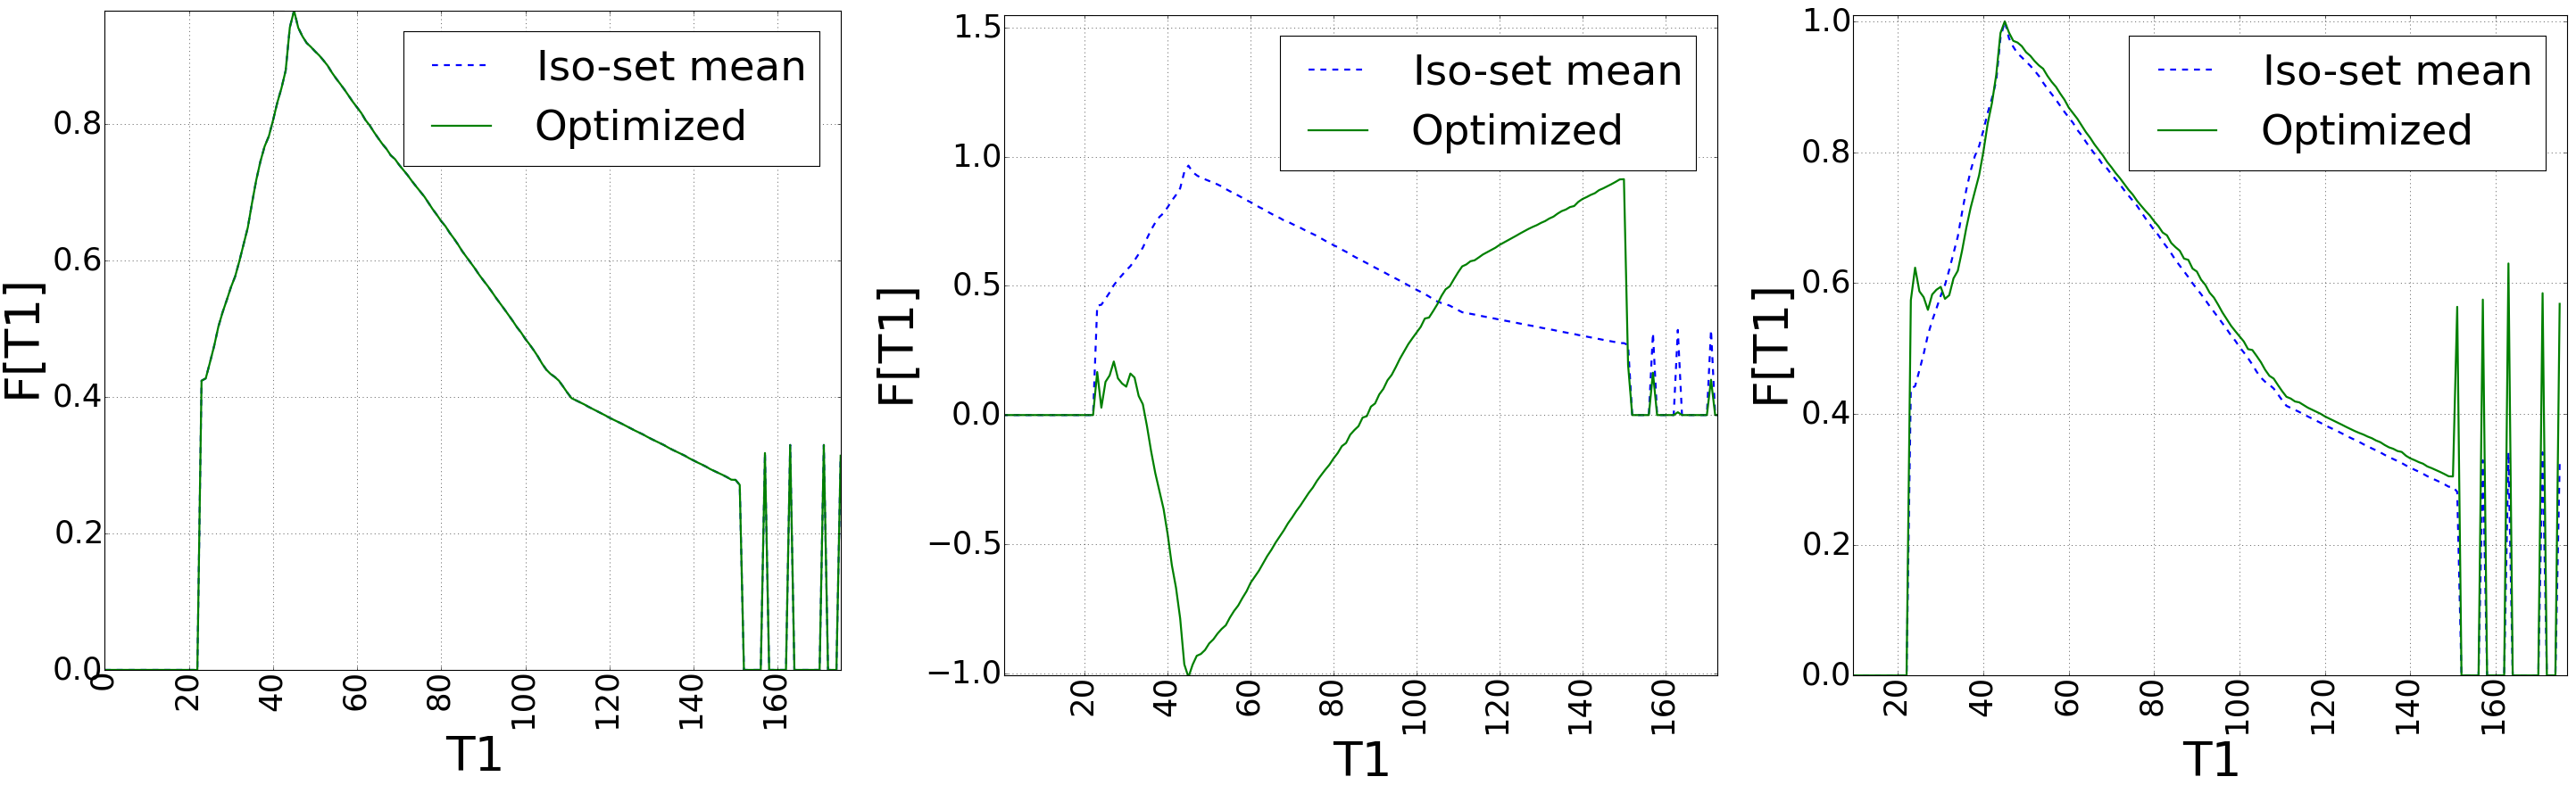
\includegraphics[width=1.0\linewidth]{images/comparison_optimal_transfers_t1lab_3_centered.png}
    \caption{{\small Comparison of optimal transfer functions maximizing \eqref{eq:ecc_neg_likelihood_vector_form} (using BFGS \cite{GVK502988711}) against the iso-set means $\mathbf{\bar{f}}$. The window size was set to radius $4$ voxels ($9\times 9\times 9$). Starting from $\mathbf{\bar{f}}$ (left), the optimized transfer stays very close to it. Initializing all elements uniformly at random in [0,1] (center), the optimized transfer function may be far from $\mathbf{\bar{f}}$, but after applying an affine transform normalizing them to $[0,1]$ (normalizing after changing the sign, in this case), the transfer functions are very similar (right). The same behaviour is observed when we compute T1 as a function of T2.}}    
\label{fig:comparison_optimal_transfers}\figcloser
\end{figure}
%\subfloat[T1 as a function of T2]{\label{fig:t2lab_comparison}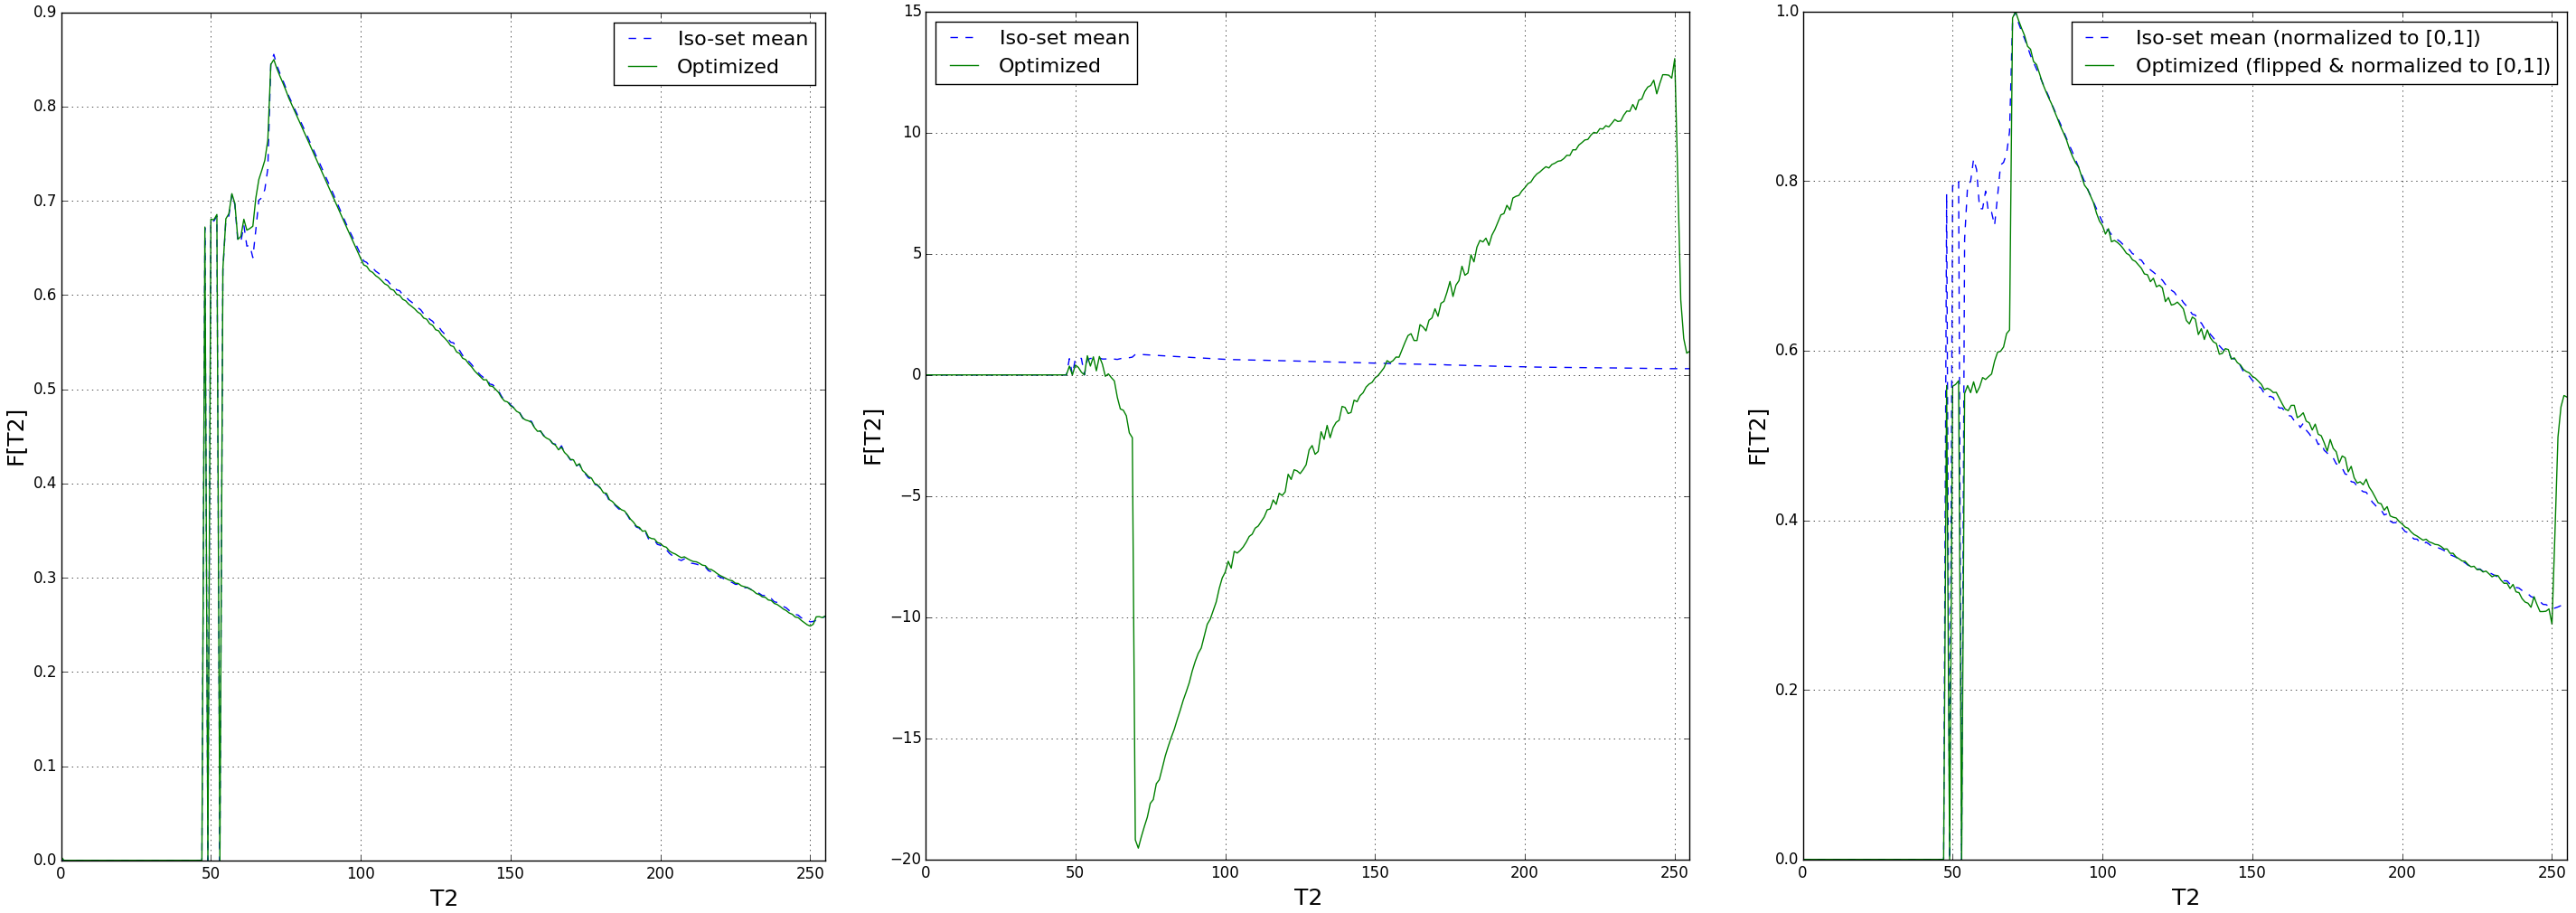
\includegraphics[width=1.0\linewidth]{images/comparison_optimal_transfers_t2lab_3.png}}\\
\begin{figure}[t]
\centering
    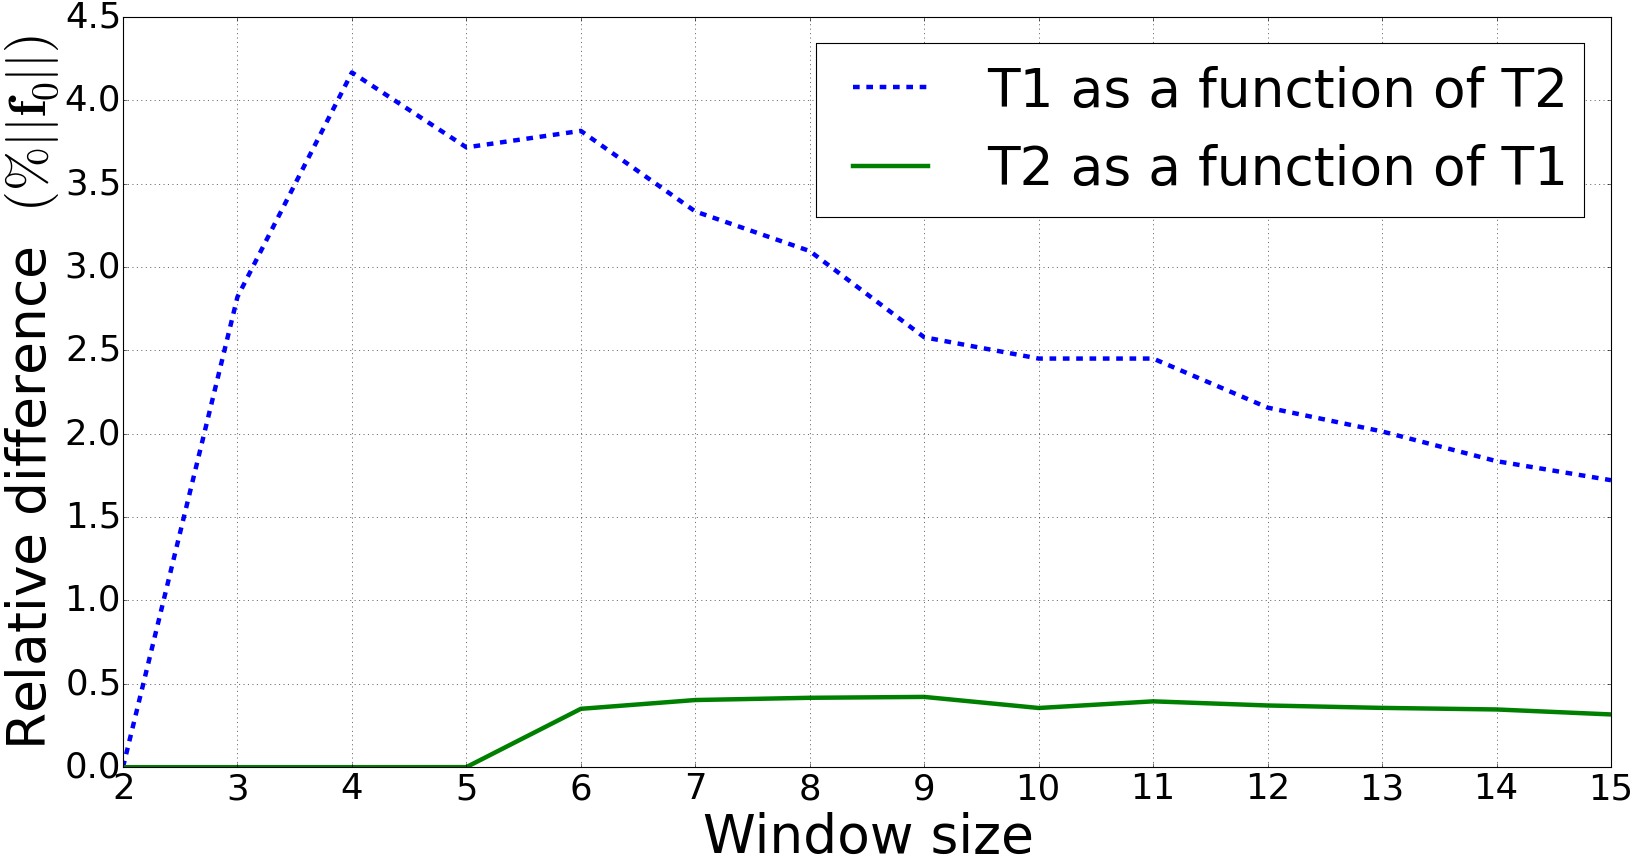
\includegraphics[width=1.0\linewidth]{images/LLR_transfer_rmse_centered.png}
    \caption{{\small Difference between $\mathbf{\bar{f}}$ and the optimal transfer function maximizing \eqref{eq:ecc_neg_likelihood_vector_form} (computed with BFGS starting from $\mathbf{\bar{f}}$) as a function of the window size $w$ (the total number voxels is $(2w+1)^{3}$). \textcolor{red}{After $w=4$, the deviation from $\mathbf{\bar{f}}$ decreases as we increase $w$.}}}
\label{fig:LLR_transfer_rmse}\figcloser
\end{figure}
In Fig. \ref{fig:ecc_test_good}, we illustrate the effect of introducing the global non-linear transfer into the local linear model\footnote{See supplementary material for an enlarged version of Fig. \ref{fig:ecc_test_good}.}. This example is the same as Fig. \ref{fig:llr_test}, the fixed image $I$ is the T1, the moving image $J$ is the T2, but instead of fitting the local linear models between $I$ and $J$ directly, we used $F[I]$ and $J$, where $F$ is defined by vector $\mathbf{\bar{f}}$. It can be observed that the non-linear local relationship was made significantly closer to linear by the use of the global transfer function.
\begin{figure}[t]
\centering
    \subfloat[]{\label{fig:FT1T2_affine_fit_scatter1}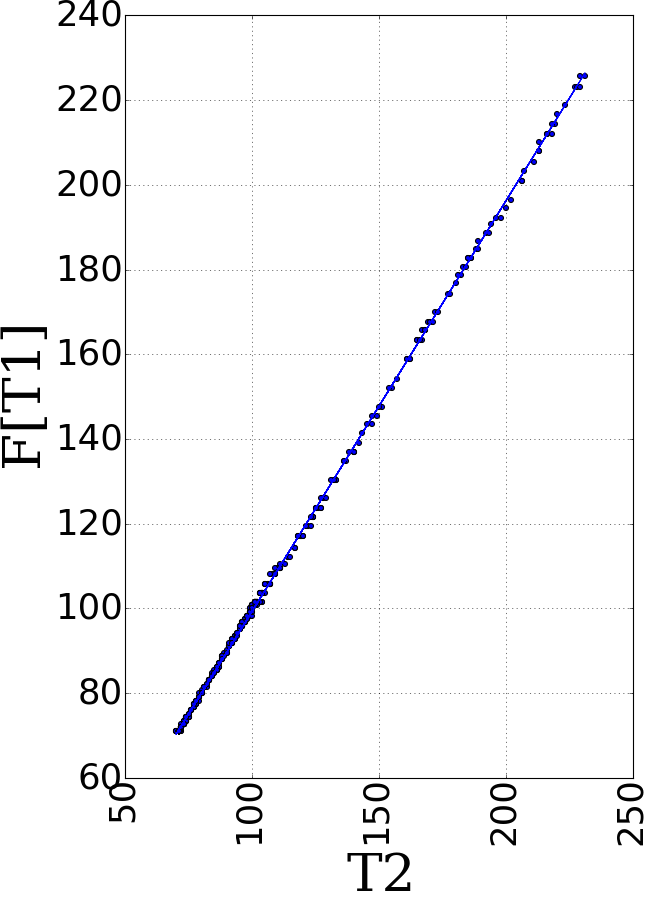
\includegraphics[width=0.2\linewidth]{images/Ft1_aafo_t2_sample2.png}}
    \subfloat[]{\label{fig:FT1T2_affine_fit_scatter2}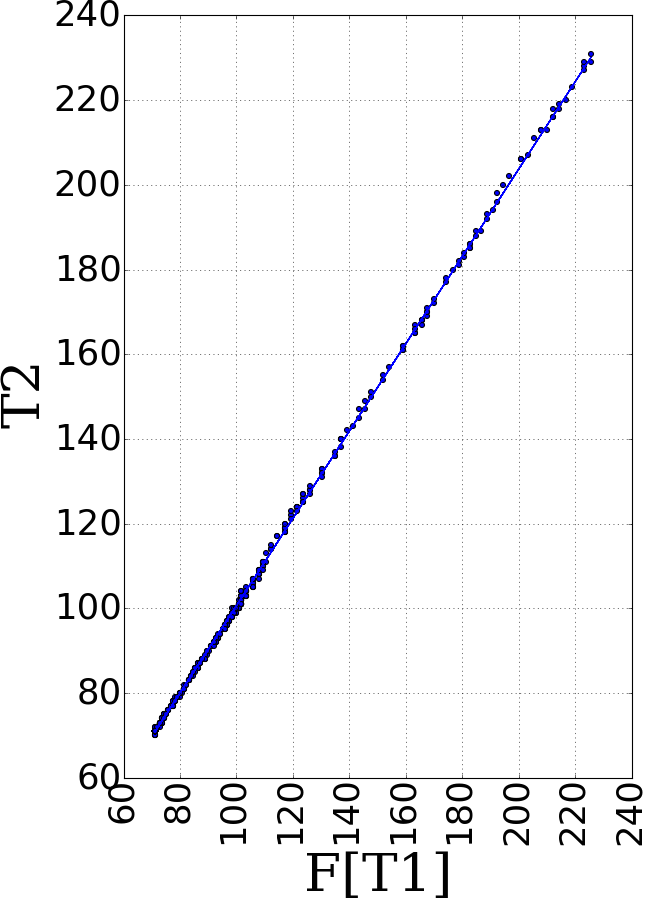
\includegraphics[width=0.2\linewidth]{images/t2_aafo_Ft1_sample2.png}}
    \subfloat[]{\label{fig:FT1T2_affine_fit_map}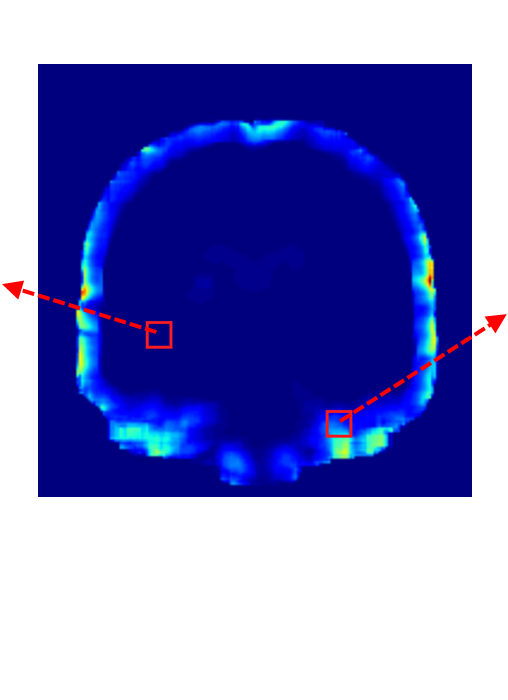
\includegraphics[width=0.2\linewidth]{images/residuals_t2_arrows.png}}
    \subfloat[]{\label{fig:FT1T2_affine_fit_scatter1}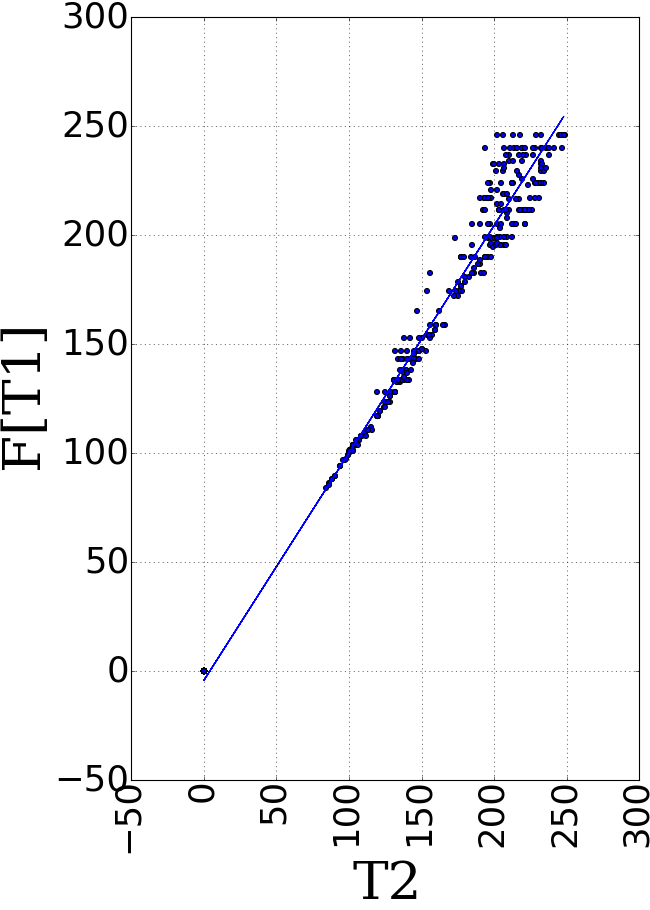
\includegraphics[width=0.2\linewidth]{images/Ft1_aafo_t2_sample1.png}}
    \subfloat[]{\label{fig:FT1T2_affine_fit_scatter2}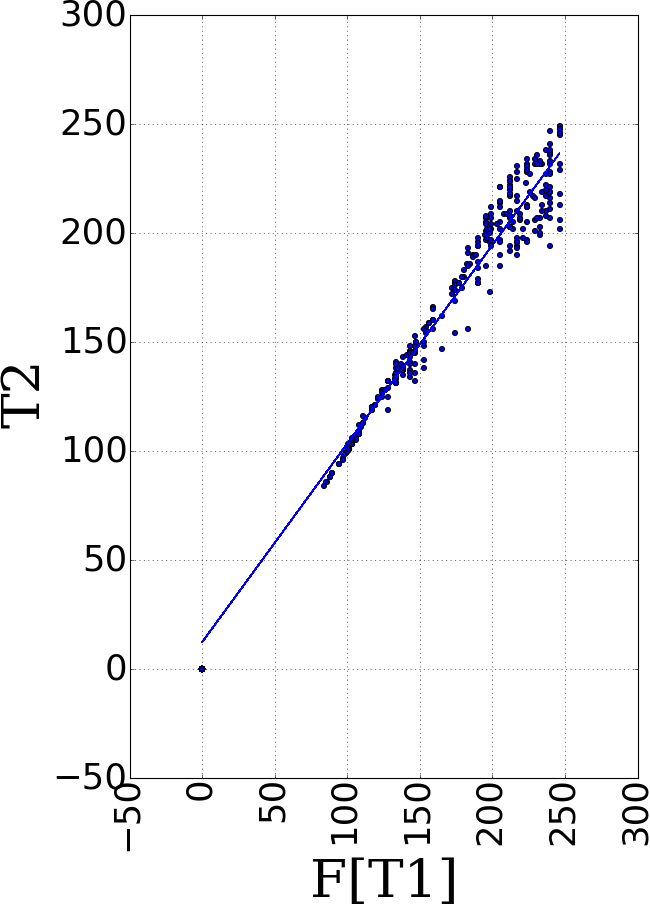
\includegraphics[width=0.2\linewidth]{images/t2_aafo_Ft1_sample1.png}}\\
    \caption{{\small Local linear reconstruction between T2 intensities and F[T1], where F is given by $\mathbf{\bar{f}}$ \eqref{eq:average_of_isosets}. Center image (c) depicts the reconstruction error in false color. The selected windows are the same as in Fig. \ref{fig:llr_test}. The local relationship was made closer to linear by applying the global non-linear transfer F.}}
\label{fig:ecc_test_good}\figcloser
\end{figure}


\subsection{Bidirectional transfer functions}
A limitation of \textcolor{red}{ using one single transfer function } is that one of the image modalities must be chosen \emph{a priori} as the target modality (either map intensities from modality A to modality B or viceversa). This is an important decision and what choice is the best may not be obvious in general. To overcome this limitation, we estimate both transfer functions between $I$ and $J$. Instead of directly computing one single transformation $\phi:\Omega_{I} \rightarrow \Omega_{J}$, we aim to find two invertible transformations (\emph{diffeomorphisms}) $\phi_{I}:\Omega_{I}\rightarrow \Omega_{R}$ and $\phi_{J}:\Omega_{J}\rightarrow \Omega_{R}$ such that the images get aligned in a reference space $\Omega_{R}$ after warping them under $\phi_{I}^{-1}$ and $\phi_{J}^{-1}$. This is exactly the same formulation as the SyN algorithm proposed by Avants {\it et al.} \cite{Avants2011}, and explained in section \ref{sec:non_linear_image_registration}, where the partial transforms $\phi_{I}, \phi_{J}$ are the middle-point diffeomorphisms of a diffeomorphic flow transforming the domains $\Omega_{I}, \Omega_{J}$ toward each other.\\
%To illustrate this, Fig. \ref{fig:ecc_test_bad} depicts the same example as Fig. \ref{fig:ecc_test_good}, but instead of mapping intensities from T1 to T2, we map intensities from T2 to T1. Although the transfer function helps, the relationship is still far from affine.
%\begin{figure}[t]
%\centering
%    \subfloat[]{\label{fig:T1FT2_affine_fit_scatter1}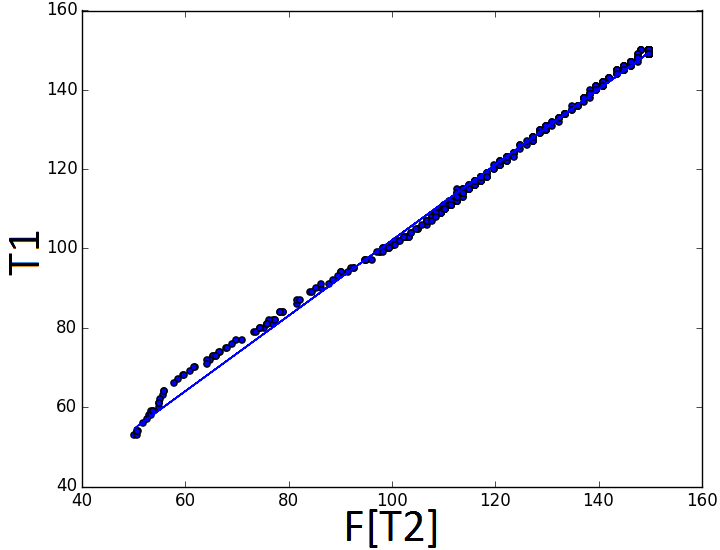
\includegraphics[width=0.2\linewidth]{images/t1_aafo_Ft2_sample2.png}}
%    \subfloat[]{\label{fig:T1FT2_affine_fit_scatter2}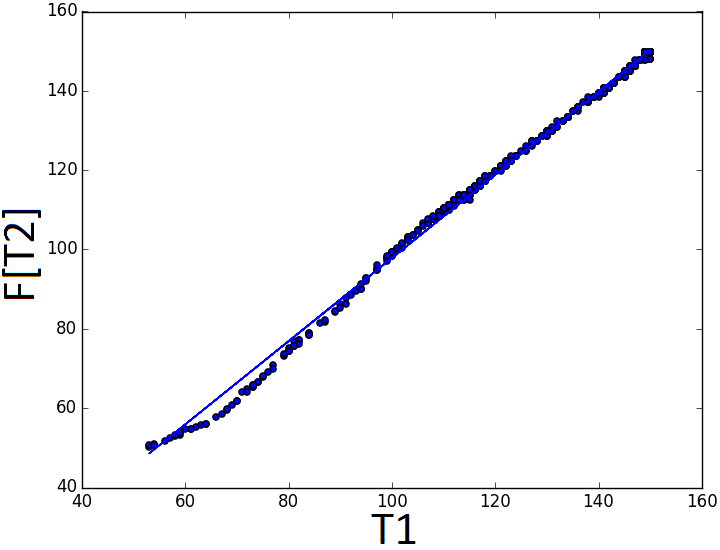
\includegraphics[width=0.2\linewidth]{images/Ft2_aafo_t1_sample2.png}}
%    \subfloat[]{\label{fig:T1FT2_affine_fit_map}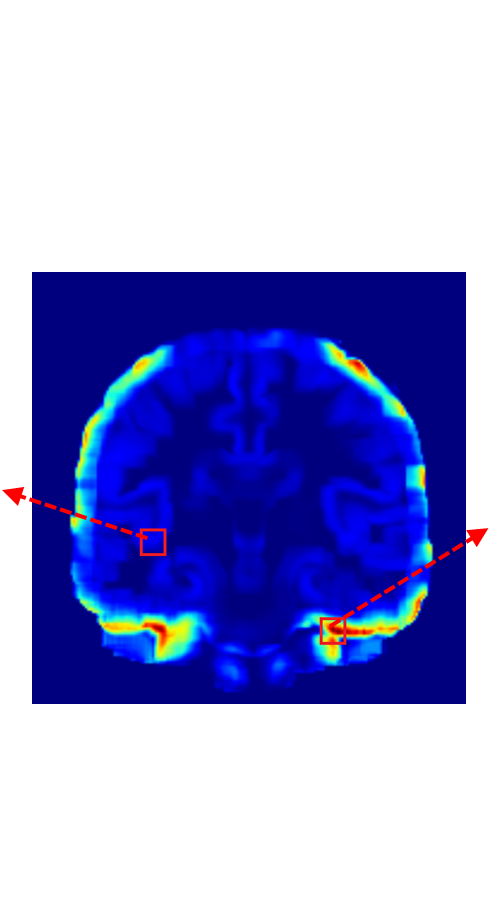
\includegraphics[width=0.2\linewidth]{images/residuals_t1_arrows.png}}
%    \subfloat[]{\label{fig:T1FT2_affine_fit_scatter1}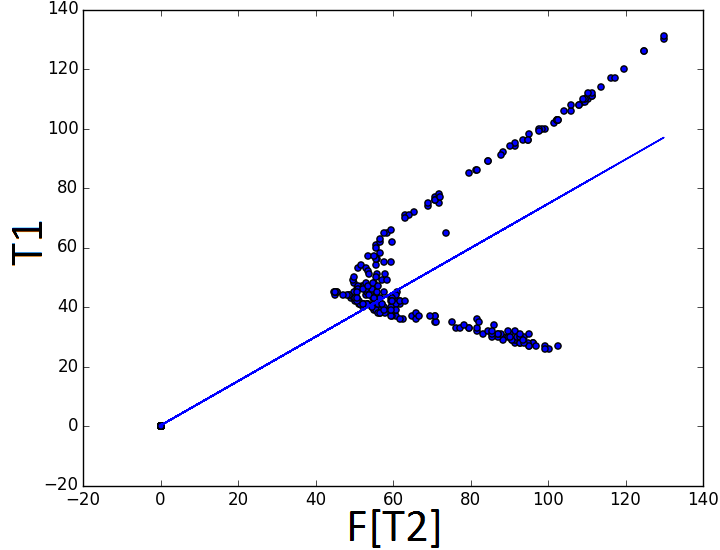
\includegraphics[width=0.2\linewidth]{images/t1_aafo_Ft2_sample1.png}}
%    \subfloat[]{\label{fig:T1FT2_affine_fit_scatter2}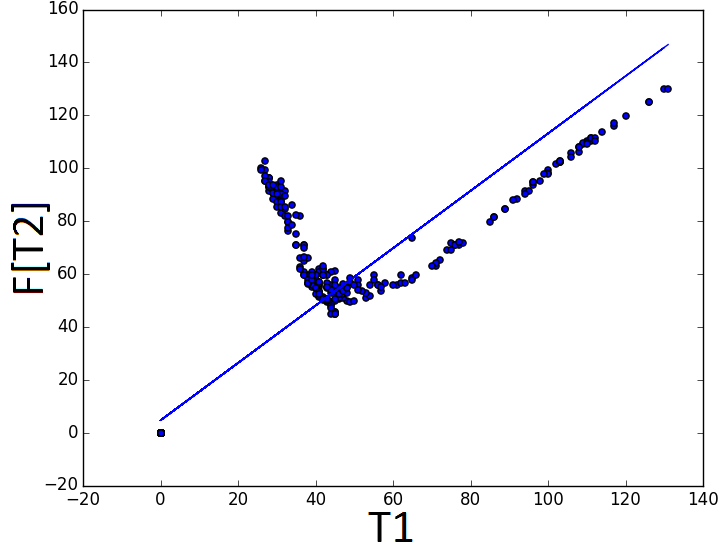
\includegraphics[width=0.2\linewidth]{images/Ft2_aafo_t1_sample1.png}}\\
%    \caption{{\small Local linear reconstruction between T1 intensities and F[T2], where F is given by $\mathbf{\bar{f}}$ \eqref{eq:average_of_isosets}. Center image (c) %depicts the reconstruction error in false color. The selected windows are the same as in Fig. \ref{fig:ecc_test_good}. The local relationship was made closer to linear by mapping %intensities from T2 to T1, but not as close as mapping from T1 to T2.}}
%\label{fig:ecc_test_bad}
%\end{figure}

%\begin{figure}[t]
%\centering
%\fbox{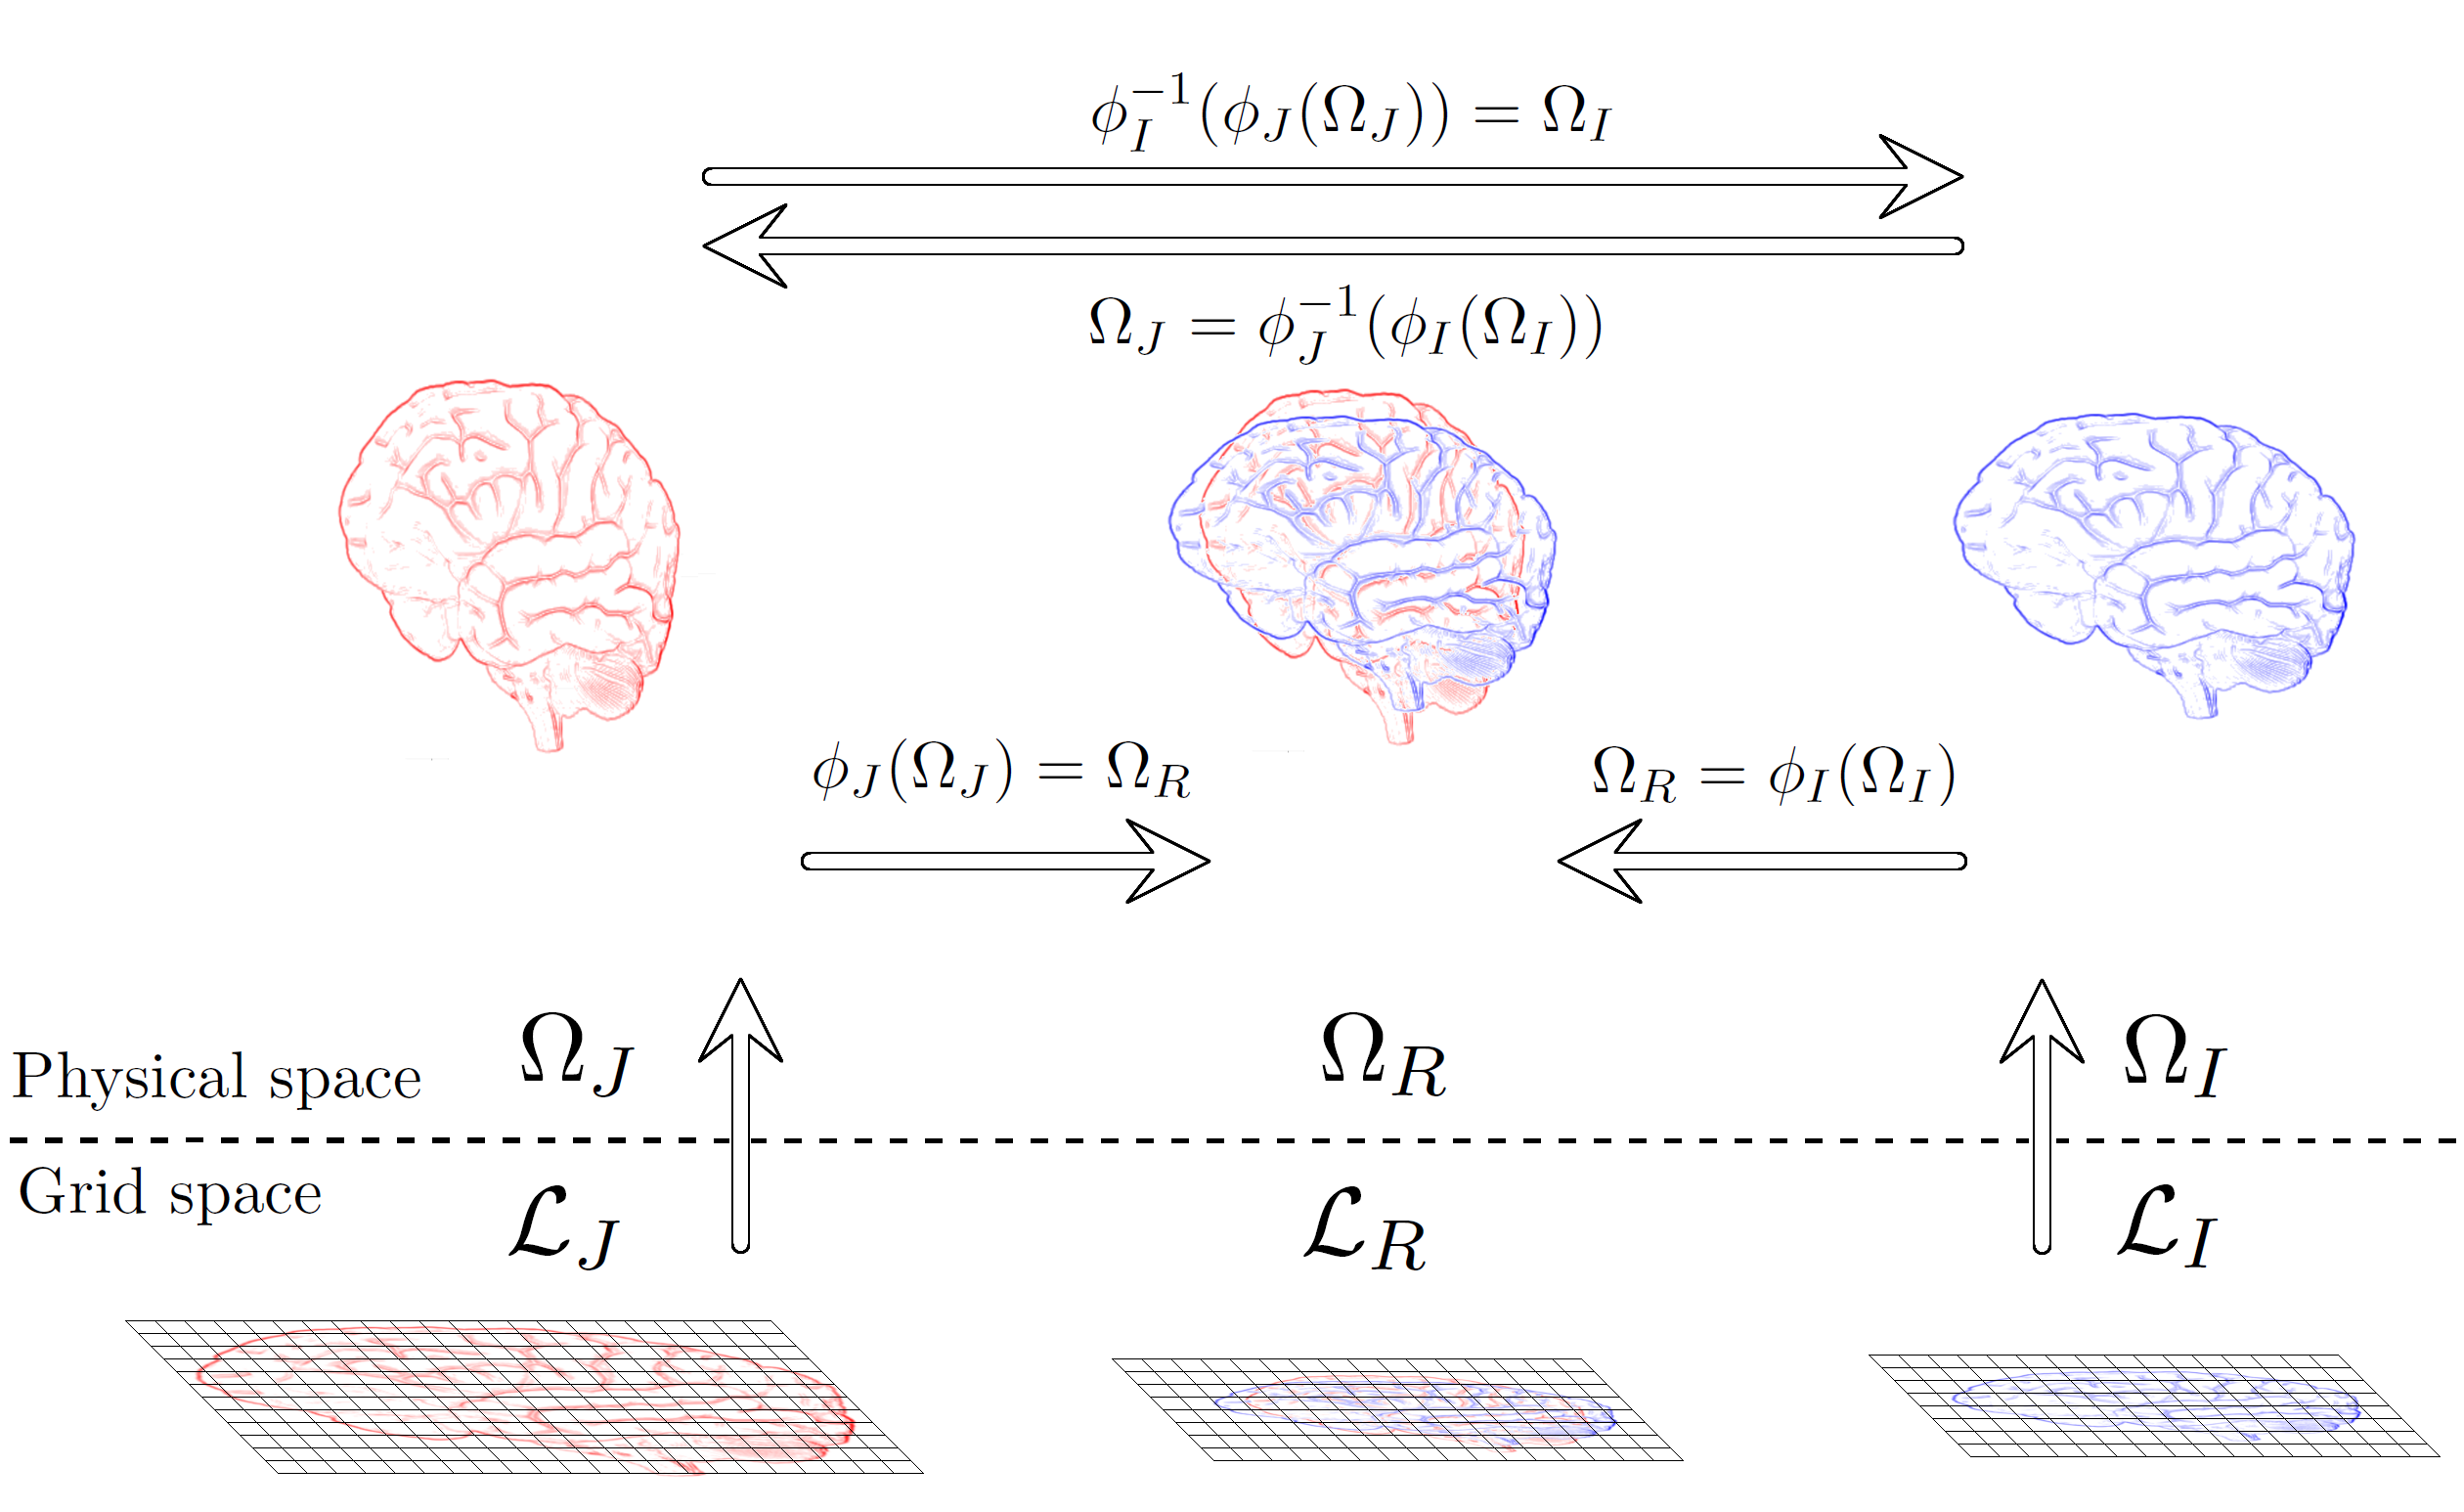
\includegraphics[width=1.0\linewidth]{images/syn_overview.png}}
%\caption{{\small The Greedy SyN algorithm registers two input images by computing two diffeomorphisms that map the input images towards a common reference domain. The final
%diffeomorphism is computed by composing the two partial diffeomorphisms.}}
%\label{fig:syn_overview}\figcloser
%\end{figure}

As before, consider a rectangular local window $W_{\mathbf{v}}$ but this time centered at a voxel $\mathbf{v}$ in the reference space $\mathbf{v}\in\Omega_{R}$. Denote by
\begin{align*}
    \mathbf{x}_{\mathbf{v}} &= \left(I(\phi_{I}^{-1}(\mathbf{v}_{1})), I(\phi_{I}^{-1}(\mathbf{v}_{2})), ..., I(\phi_{I}^{-1}(\mathbf{v}_{n}))\right)^{T}\\
    \mathbf{y}_{\mathbf{v}} &= \left(J(\phi_{J}^{-1}(\mathbf{v}_{1})), J(\phi_{J}^{-1}(\mathbf{v}_{2})), ..., J(\phi_{J}^{-1}(\mathbf{v}_{n}))\right)^{T},
\end{align*}
the images $I, J$ evaluated at all voxels of the local window $\mathbf{v}_{i}\in W_{\mathbf{v}}, i=1, 2, .., n$. Note that this time, both vectors $\mathbf{x}_{\mathbf{v}}$ and $\mathbf{y}_{\mathbf{v}}$ are moving according to the (inverses of the) transforms $\phi_{I}$ and $\phi_{J}$. By introducing both transfer functions, $F_{I}$ and $F_{J}$ mapping intensities from $I$ to $J$ and from $J$ to $I$ respectively, our symmetric model may be written as follows:
\begin{equation}\label{eq:symmetric_ecc_model}
    \begin{array}{ccccc}
        \widehat{\mathbf{y_v}} = \left[F_{I}\left[\mathbf{x}_{\mathbf{v}}\right] \; \mathbbm{1}\right]\boldsymbol{\alpha} + \eta_{I}(\mathbf{v}) \; \forall \mathbf{v}\in\Omega_{R}\\
        \widehat{\mathbf{x_v}} = \left[F_{J}\left[\mathbf{y}_{\mathbf{v}}\right] \; \mathbbm{1}\right]\boldsymbol{\beta} + \eta_{J}(\mathbf{v}) \; \forall \mathbf{v}\in\Omega_{R}\\
    \end{array},
\end{equation}
\textcolor{red}{where $\widehat{\mathbf{x_v}}$ and $\widehat{\mathbf{y_v}}$ are centered and normalized, as before}. By assuming independence between the two sets of normally distributed random vectors $\eta_{I}$ and $\eta_{I}$, it follows immediately that maximizing the log-likelihood of model \eqref{eq:symmetric_ecc_model} is equivalent to maximizing the (symmetric) ECC matching functional:
\begin{equation*}
    ECC(I, J;\phi_{I}, \phi_{J}) = CC(\mathbbm{E}[J|I], J ; \phi_{J}) + CC(\mathbbm{E}[I|J], I ; \phi_{I}).
\end{equation*}
This functional can be easily incorporated into the SyN transformation model by computing $F_{I}$ and $F_{J}$ at each iteration (after line 4 in Algorithm \ref{alg:Greedy_SyN}) and use them to evaluate the gradient of $ECC(I, J;\phi_{I}, \phi_{J})$\footnote{See supplementary material for a complete description of the algorithm.}.
%the negative log likelyhood is proportional to
%\begin{displaymath}
%    U(I, J;\phi) =
%    \sum_{v\in\Omega_{R}}\left(1-\frac{\left(F_{I}\left[\mathbf{x}_{v}\right]^{T} \mathbf{y}_{v}\right)^{2}}{||F_{I}\left[\mathbf{x}_{v}\right]||^{2}||\mathbf{y}_{v}||^{2}}\right) %+
%    \left(1-\frac{\left(F_{J}\left[\mathbf{y}_{v}\right]^{T} \mathbf{x}_{v}\right)^{2}}{||F_{J}\left[\mathbf{y}_{v}\right]||^{2}||\mathbf{x}_{v}||^{2}}\right),
%\end{displaymath}
%and the m.l.e. for $\phi_{I}$ and $\phi_{J}$ can be obtain by maximizing the symmetric Expected Cross Correlation:
%\begin{equation}
%    ECC(I, J;\phi) =
%    \sum_{v\in\Omega_{R}}\frac{\left(F_{I}\left[\mathbf{x}_{v}\right]^{T} \mathbf{y}_{v}\right)^{2}}{||F_{I}\left[\mathbf{x}_{v}\right]||^{2}||\mathbf{y}_{v}||^{2}} +
%    \frac{\left(F_{J}\left[\mathbf{y}_{v}\right]^{T} \mathbf{x}_{v}\right)^{2}}{||F_{J}\left[\mathbf{y}_{v}\right]||^{2}||\mathbf{x}_{v}||^{2}}
%\end{equation}



\iffalse
\begin{figure}[t]
    \subfloat[]{\label{fig:epicor_b0up_ecc.png}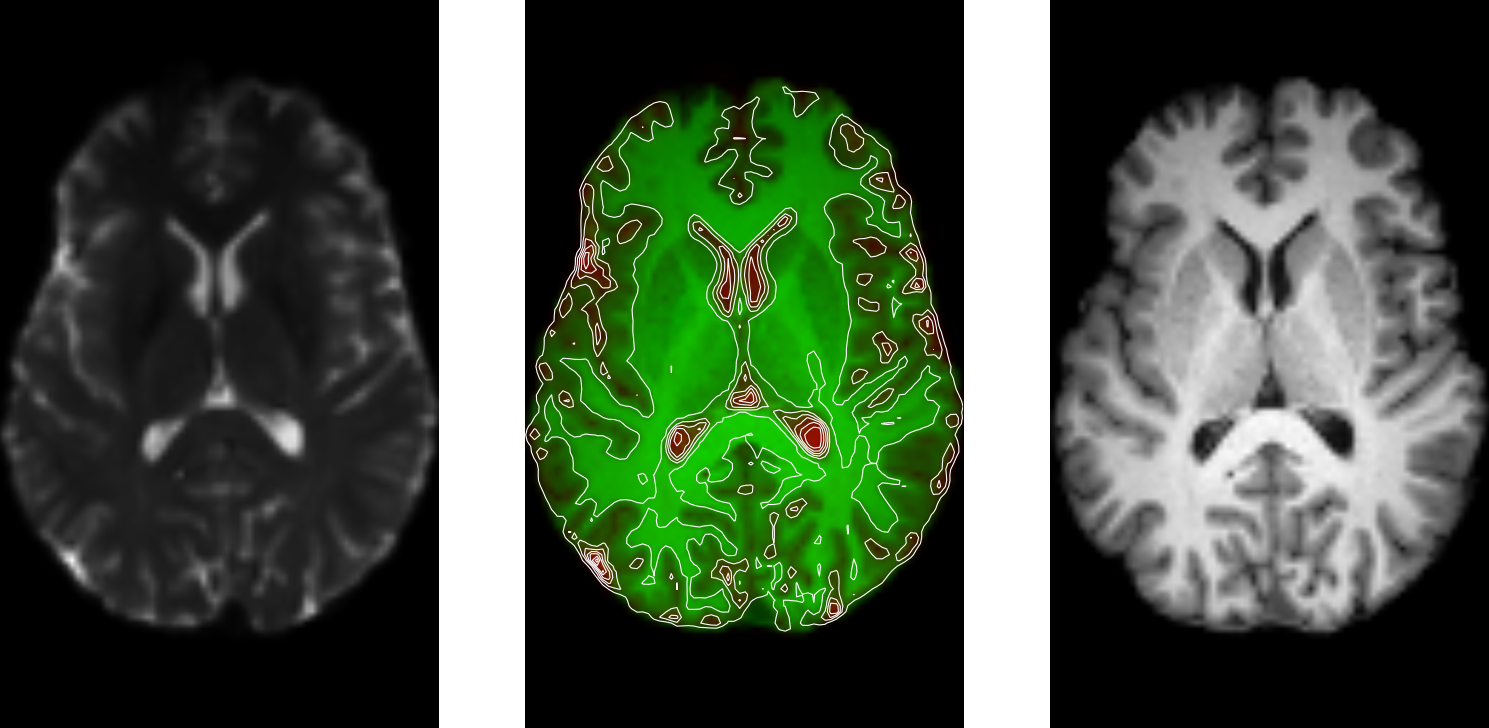
\includegraphics[width=1\linewidth]{images/T1B0Result/epicor_b0up_ecc.png}}\\
    \subfloat[]{\label{fig:epicor_b0up_mi.png}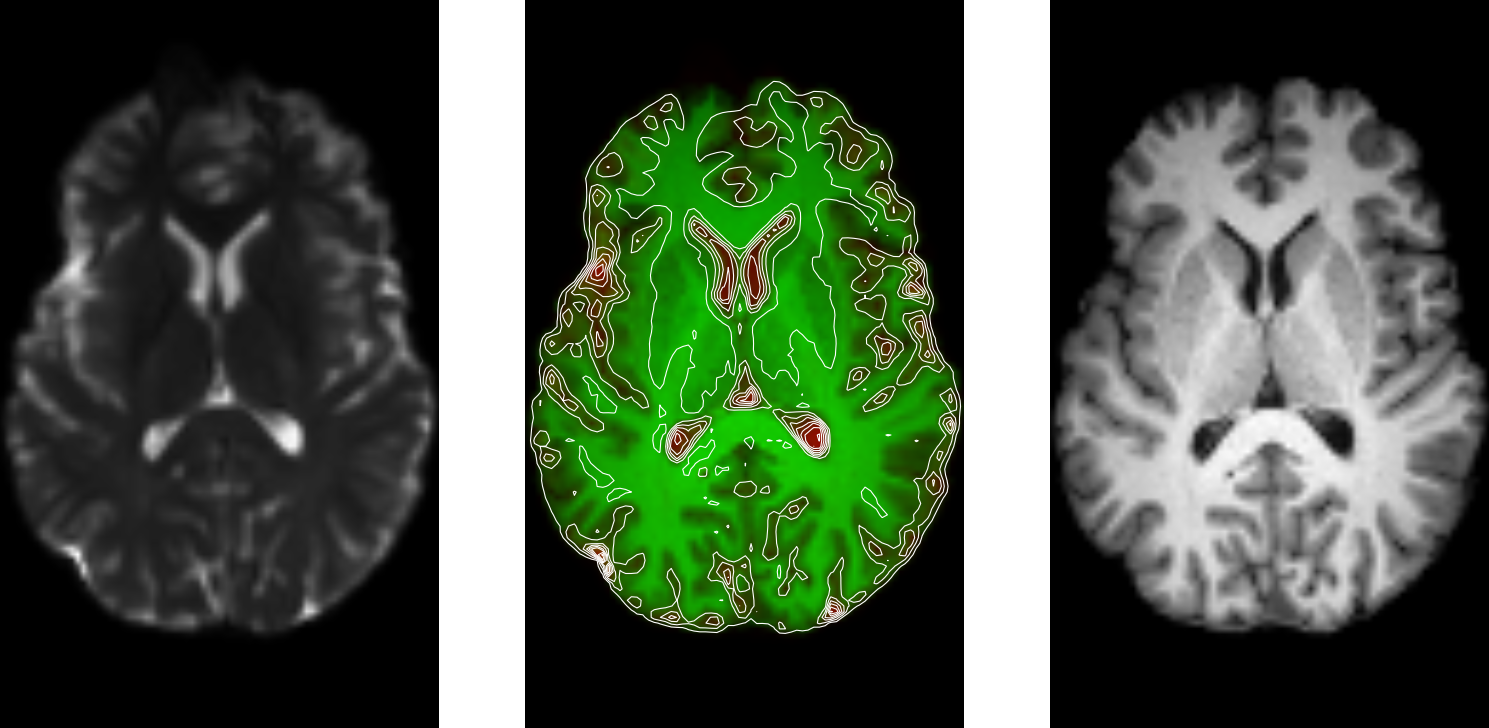
\includegraphics[width=1\linewidth]{images/T1B0Result/epicor_b0up_mi.png}}\\
    \caption{{\small Registration of B0(blip up) to T1.}}
\label{fig:epicor_up_ecc}\figcloser
\end{figure}

\begin{figure}[t]
\centering
    \subfloat[]{\label{fig:b0_up_sagital_zoom}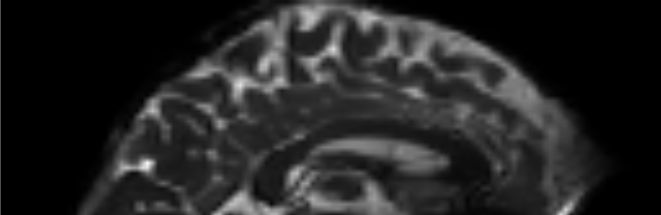
\includegraphics[width=0.5\linewidth]{images/T1B0Result/b0_up_sagital_zoom.png}}
    \subfloat[]{\label{fig:affine_mi_t1b0up_sagital_zoom.png}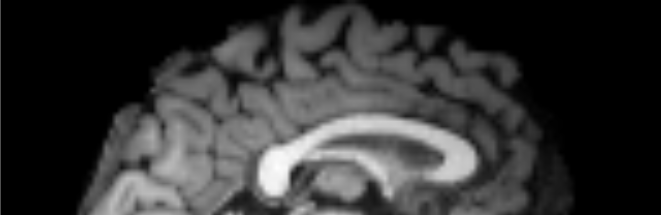
\includegraphics[width=0.5\linewidth]{images/T1B0Result/affine_mi_t1b0up_sagital_zoom.png}}\\
    \subfloat[]{\label{fig:synecc_contours_t1b0up_sagital_zoom}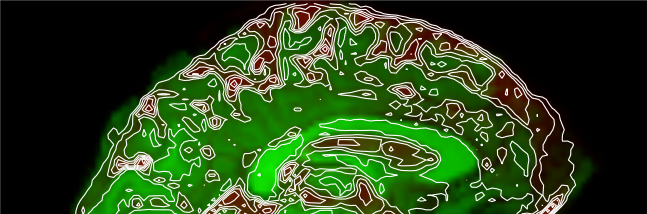
\includegraphics[width=0.5\linewidth]{images/T1B0Result/synecc_contours_t1b0up_sagital_zoom.png}}
    \subfloat[]{\label{fig:synmi_contours_t1b0up_sagital_zoom}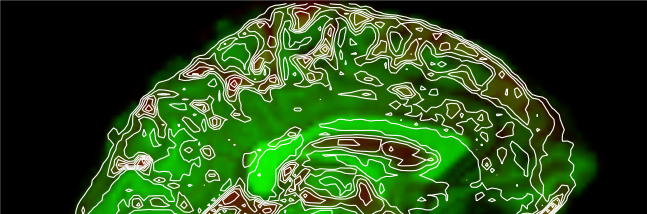
\includegraphics[width=0.5\linewidth]{images/T1B0Result/synmi_contours_t1b0up_sagital_zoom.png}}\\
    \subfloat[]{\label{fig:synecc_t1b0up_sagital_zoom}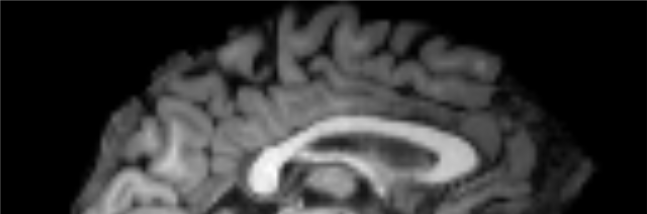
\includegraphics[width=0.5\linewidth]{images/T1B0Result/synecc_t1b0up_sagital_zoom.png}}
    \subfloat[]{\label{fig:synmi_t1b0up_sagital_zoom}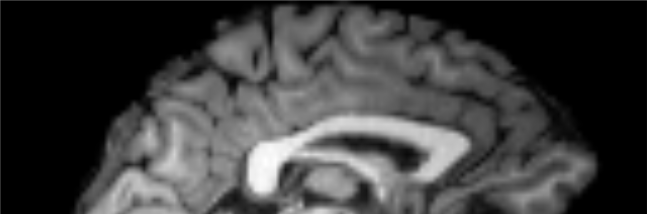
\includegraphics[width=0.5\linewidth]{images/T1B0Result/synmi_t1b0up_sagital_zoom.png}}\\
    \caption{{\small Registration of T1 to $B_0$ (blip up).}}
\label{fig:sagital_zoom_t1b0up}\figcloser
\end{figure}


\begin{figure}[t!]
    \subfloat[]{\label{fig:epicor_b0down_ecc.png}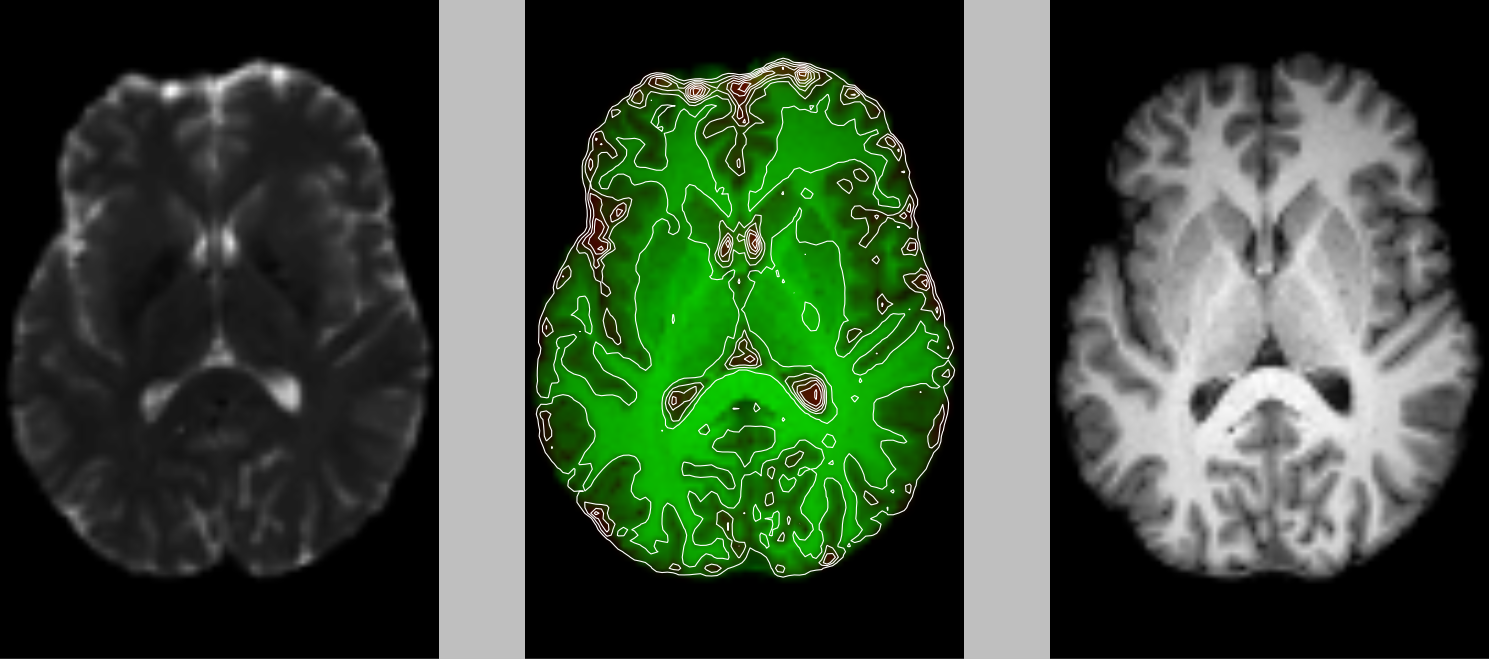
\includegraphics[width=1\linewidth]{images/T1B0Result/epicor_b0down_ecc.png}}\\
    \subfloat[]{\label{fig:epicor_b0down_mi.png}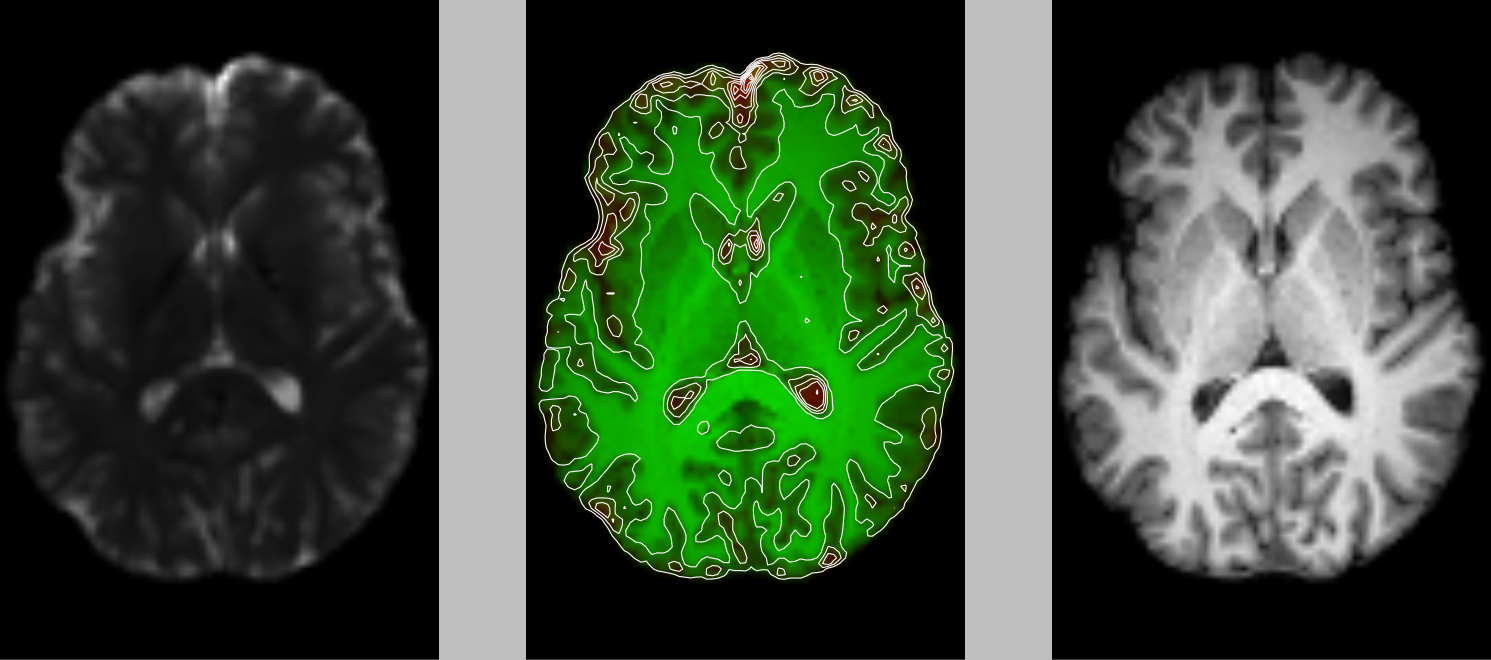
\includegraphics[width=1\linewidth]{images/T1B0Result/epicor_b0down_mi.png}}\\
    \caption{Registration of $B0$ (blip up) to T1.}
\label{fig:epicor_down_ecc}\figcloser
\end{figure}

\begin{figure}[t!]
\centering
    \subfloat[]{\label{fig:b0_down_sagital_zoom}
\includegraphics[width=0.5\linewidth]{images/T1B0Result/b0_down_sagital_zoom.png}}
    \subfloat[]{\label{fig:t1_sagital_zoom}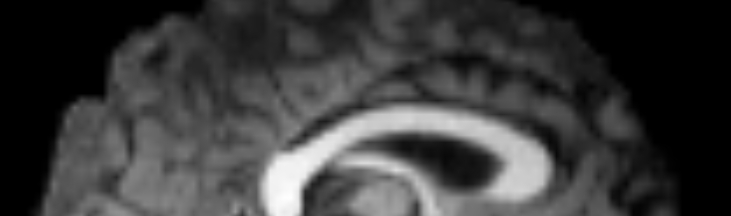
\includegraphics[width=0.5\linewidth]{images/T1B0Result/t1_sagital_zoom.png}}\\
    \subfloat[]{\label{fig:synecc_contours_t1b0_sagital_zoom}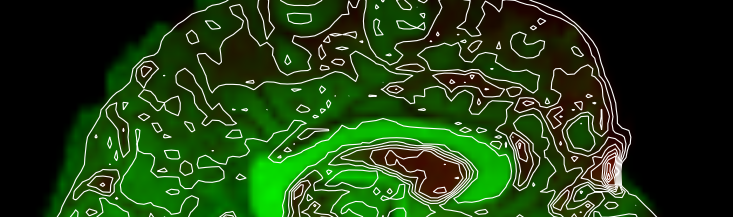
\includegraphics[width=0.5\linewidth]{images/T1B0Result/synecc_contours_t1b0_sagital_zoom.png}}
    \subfloat[]{\label{fig:synmi_contours_t1b0_sagital_zoom}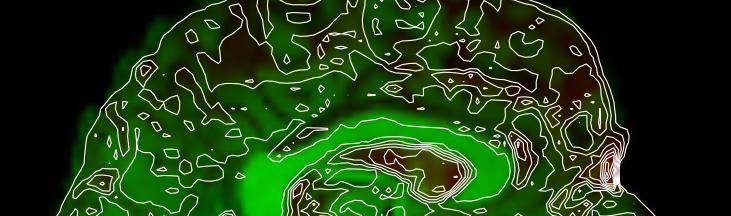
\includegraphics[width=0.5\linewidth]{images/T1B0Result/synmi_contours_t1b0_sagital_zoom.png}}\\
    \subfloat[]{\label{fig:synecc_t1b0_sagital_zoom}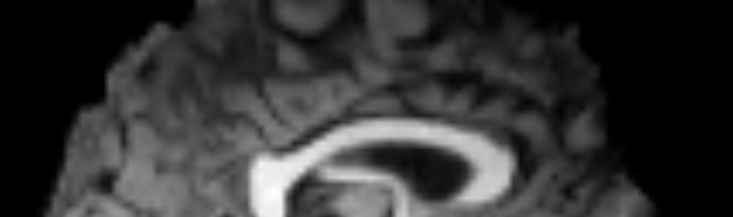
\includegraphics[width=0.5\linewidth]{images/T1B0Result/synecc_t1b0_sagital_zoom.png}}
    \subfloat[]{\label{fig:synmi_t1b0_sagital_zoom}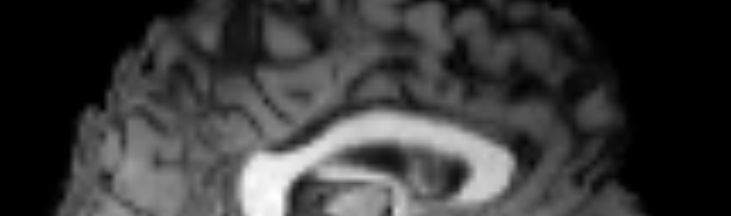
\includegraphics[width=0.5\linewidth]{images/T1B0Result/synmi_t1b0_sagital_zoom.png}}\\
    \caption{Registration of T1 to $B_0$ (blip down).}
\label{fig:sagital_zoom_t1b0down}\figcloser
\end{figure}


\begin{figure}[t!]
    \subfloat[]{\label{fig:jaccard_T1_B0}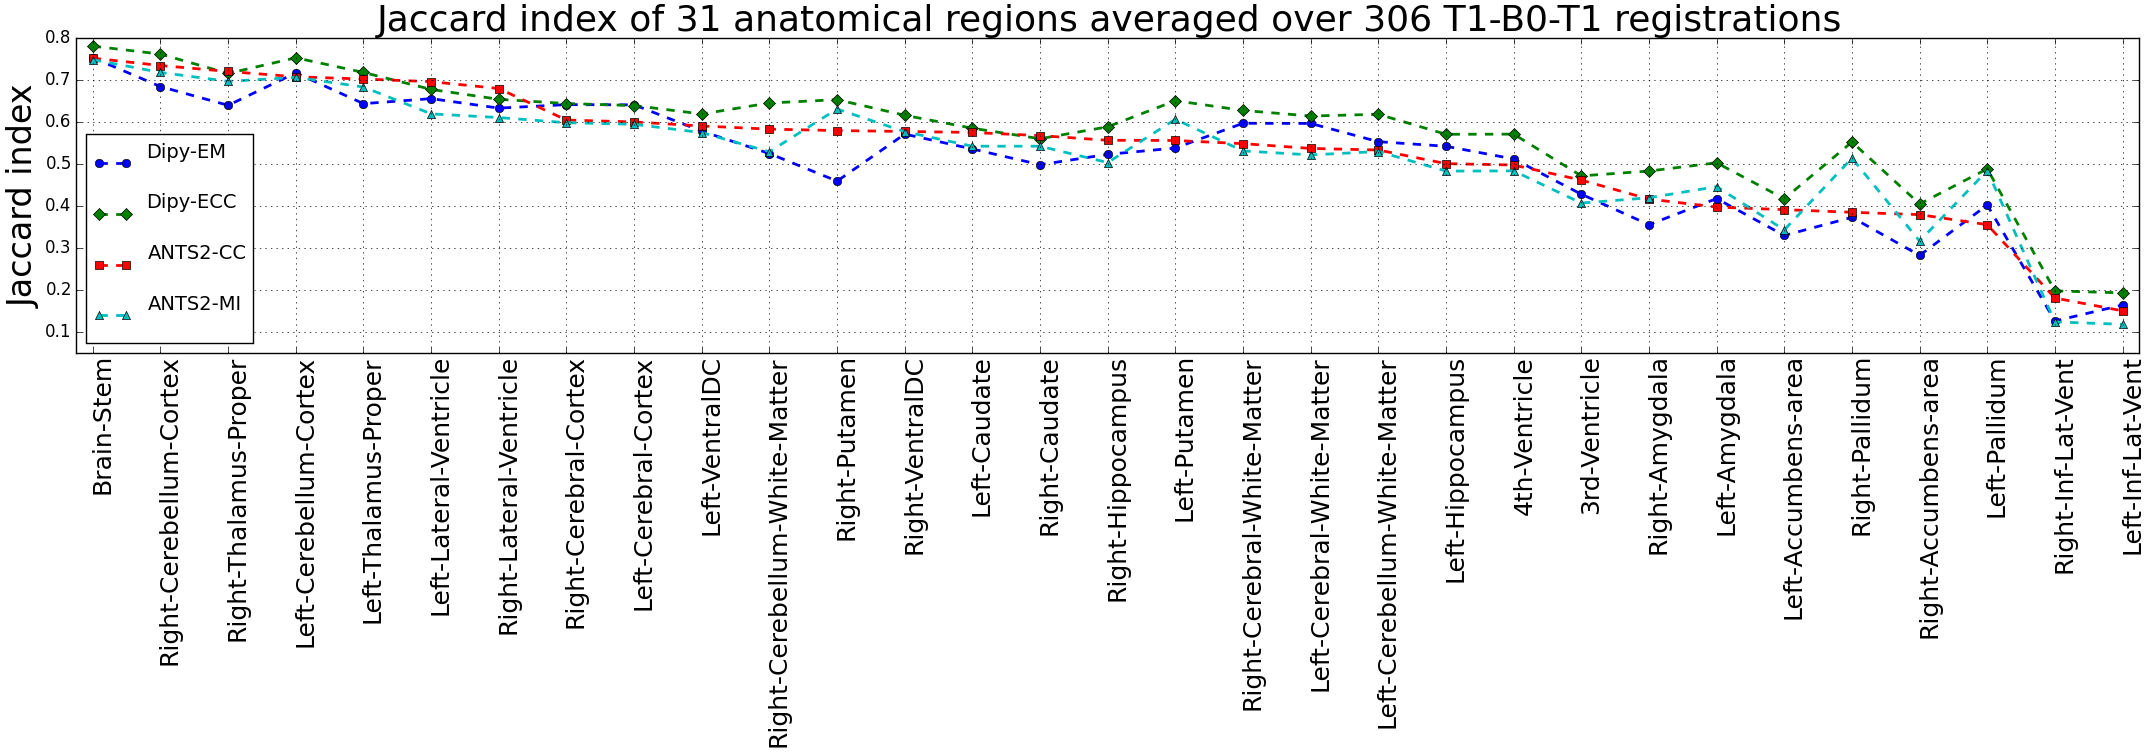
\includegraphics[width=1\linewidth]{images/T1B0Result/jaccard_T1_B0.png}}\\
    \subfloat[]{\label{fig:jaccard_boxplots_T1_B0}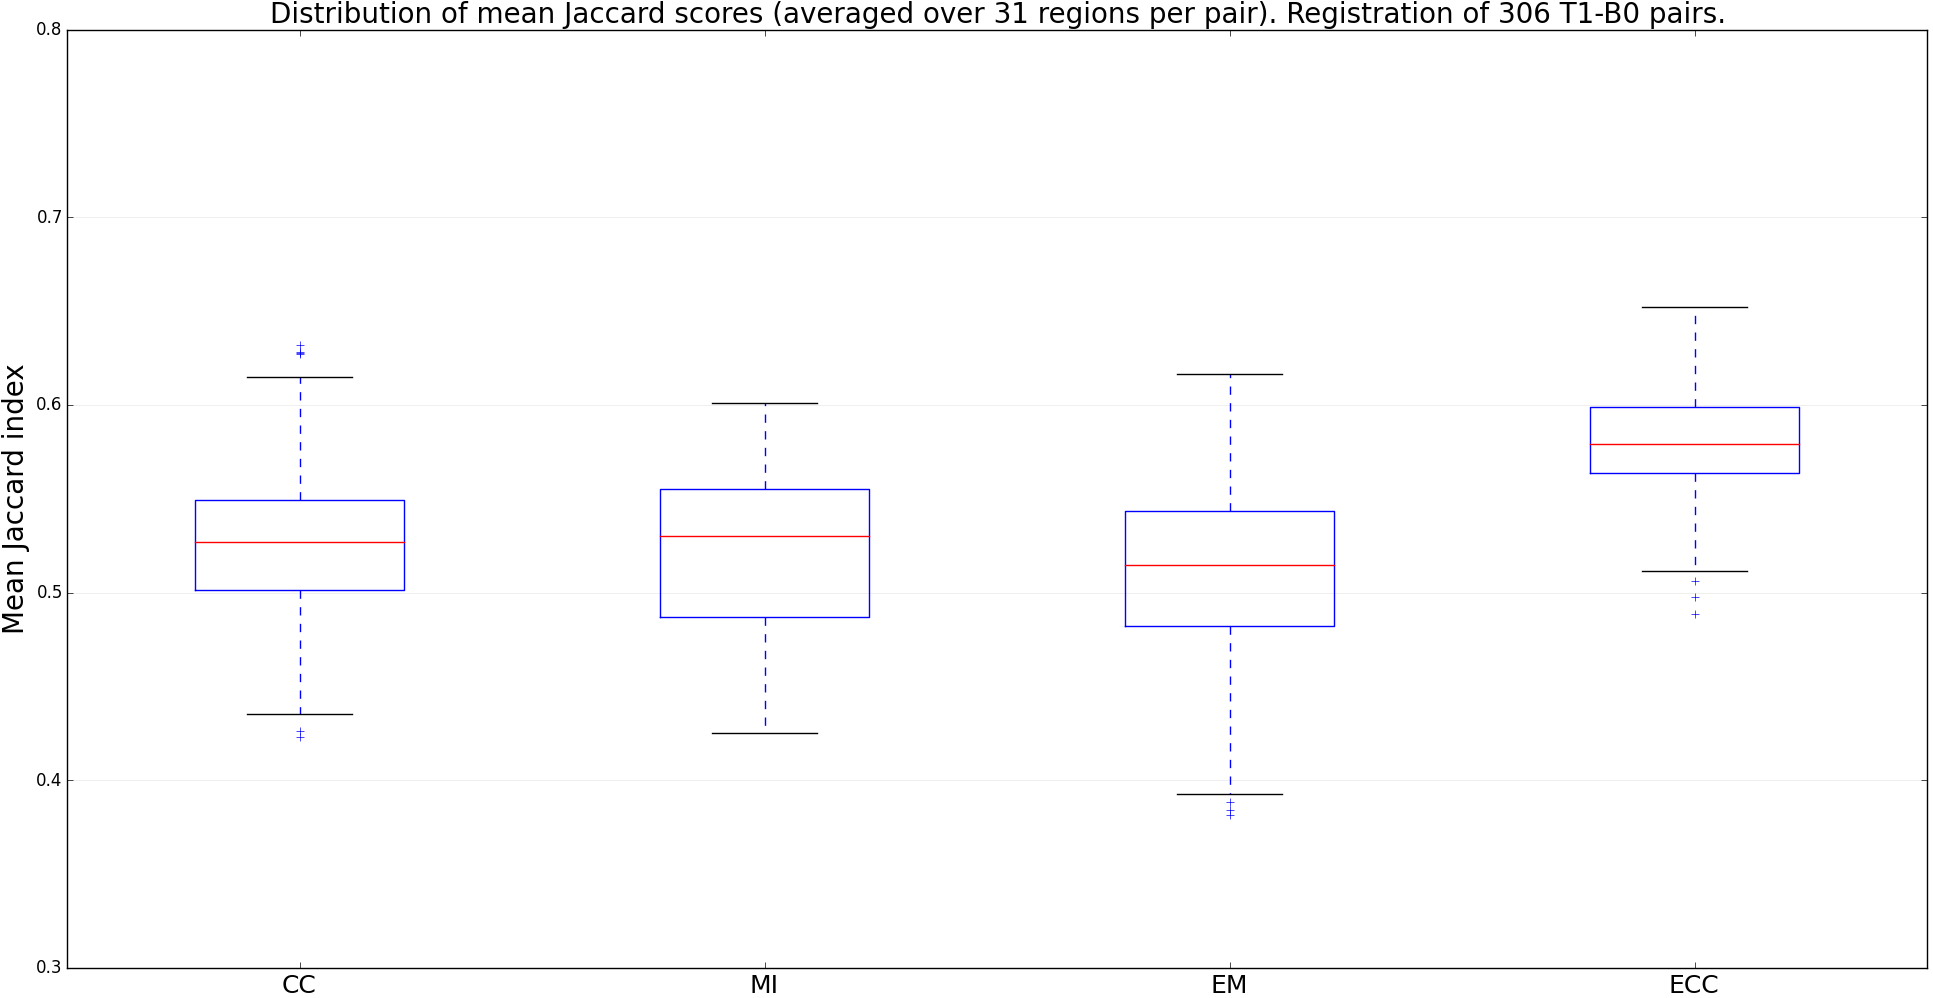
\includegraphics[width=1\linewidth]{images/T1B0Result/jaccard_boxplots_T1_B0.png}}\\
    \caption{Registration result of $B_0$ (blip down) to T1.}
\label{fig:epicor_down_ecc}\figcloser
\end{figure}

\fi 